%%
%% Elsevier CAS single-column manuscript (converted from IEEE Access draft)
%%
\documentclass[a4paper,fleqn]{cas-sc}

\usepackage[authoryear,longnamesfirst]{natbib}
\usepackage{amsmath,amssymb,amsfonts}
\usepackage{graphicx}
\usepackage{textcomp}
\usepackage{booktabs}
\usepackage{array}
\usepackage{tabularx}
\usepackage{float}
\usepackage{algorithm}
\usepackage{algpseudocode}
\algrenewcommand{\algorithmicindent}{1em}
\usepackage{enumitem}
\usepackage[utf8]{inputenc}
\usepackage[english]{babel}
\usepackage{hyperref}
\hypersetup{colorlinks=true, linkcolor=blue, filecolor=black, urlcolor=cyan}
\usepackage{caption}
\usepackage{pifont}
\usepackage{listings}
\usepackage{xcolor}
\usepackage{placeins}

\colorlet{cfgB}{blue!75!black}
\colorlet{cfgC}{orange!85!black}
\colorlet{cfgD}{teal!75!black}
\lstdefinelanguage{ProVerif}{%
  morekeywords={fun,reduc,equation,event,query,free,type,channel,%
    forall,let,in,if,then,else,new,out,process,phase,not,data,%
    private,bitstring,attacker,inj,true,false},
  sensitive=true,
  morecomment=[s]{(*}{*)}}
\lstset{%
  language=ProVerif,
  basicstyle=\small\ttfamily\color{black},
  keywordstyle=\bfseries\color{blue!90!black},
  commentstyle=\color{green!45!black}\itshape,
  stringstyle=\color{orange!80!black},
  backgroundcolor=\color{gray!8},
  frame=single,
  rulecolor=\color{black!40},
  framesep=4pt,
  xleftmargin=4pt,
  xrightmargin=4pt,
  framexleftmargin=4pt,
  breaklines=true,
  columns=flexible,
  keepspaces=true,
  showstringspaces=false,
  aboveskip=6pt,
  belowskip=4pt,
  captionpos=b}

\graphicspath{{figs/}}

\begin{document}
\let\WriteBookmarks\relax
\def\floatpagepagefraction{1}
\def\textpagefraction{.001}

\shorttitle{Post-Quantum Migration Paths for Consumer RSP}

\shortauthors{Lastre}

\title[mode = title]{Post-Quantum Migration Paths for Consumer Remote SIM Provisioning: Protocol Verification, Benchmarks, and Deployment Outlook}

\tnotemark[1]
\tnotetext[1]{This work evaluates the performance impact, formal
security guarantees, and deployment feasibility of post-quantum
cryptography within the GSMA SGP.22 Consumer Remote SIM Provisioning
protocol. No external funding to declare.}

\author[1]{Jhury Kevin Lastre}
\cormark[1]
\ead{lavelliane@kookmin.ac.kr}

\affiliation[1]{organization={Kookmin University},
            addressline={Department of Cybersecurity},
            city={Seoul},
            country={Republic of Korea}}

\cortext[cor1]{Corresponding author}

\begin{abstract}
The GSMA SGP.22 Consumer Remote SIM Provisioning standard uses ECDSA,
ECDH, and X.509 certificate chains, all broken by Shor's algorithm on a
cryptographically relevant quantum computer. Harvest-now-decrypt-later
(HNDL) lets recorded ES9+ traffic be decrypted later, exposing long-lived
IMSI values and credentials. Whether NIST ML-KEM (FIPS 203) and ML-DSA
(FIPS 204) fit eUICC hardware below 500 KB RAM and metered ES9+ links has
not been evaluated at full Consumer RSP scope. To our knowledge, we
present the first evaluation that jointly addresses formal verification
under classical and quantum adversaries, hardware-gap benchmarking on a
production eUICC and an STM32 Nucleo-F446RE (Cortex-M4), and four
migration configurations (a--d) for Consumer RSP, using ProVerif 2.05 under
the symbolic Dolev-Yao model with a Shor oracle in the quantum setting.
Under the quantum adversary with the Shor oracle scoped to ECDH inversion
(modelling HNDL on session keys), configurations (a) and (b) fail Q3, Q4, and
Q6; configurations (c) and (d) pass all six SGP.22 security properties in
that model. A complete Shor capability including ECDSA forgery would break
Q1 and Q2 for (a)--(c), leaving only configuration~(d) with all six properties. Configuration (c) replaces ECDH with ML-KEM-768,
retains ECDSA, and closes the HNDL threat on session keys without CI
re-issuance; configuration (d) adds ML-DSA-44, but its 16,256-byte chain
exceeds current eUICC volatile memory for full buffering, requiring
streaming certificate verification and new silicon. Mean end-to-end
session wall time is 25.20~s; TLS handshake bytes grow by a factor of
$2.4$. ML-KEM-768 key agreement overhead at step~21a was directly measured
at 0.55~ms on a software eUICC protocol flow (upper bound, x86\_64), with
full session overhead of 764~ms relative to the classical baseline; the
normalised eUICC projection ranges from [Y]~ms to [Z]~ms. Results show that
PQ-TLS transport imposes zero measurable latency overhead on RSP sessions
($p > 0.9$), while configuration (b) does not close the HNDL window, as empirically
confirmed by observing both ECDH ephemeral public keys
in plaintext on the eUICC-to-LPA APDU channel during a PQ-TLS protected
session. We recommend phased migration:
deploy (b) for transport hardening, prioritise (c) on the next eUICC
generation to close HNDL, and target (d) once SGP.22 specifies streaming
verification and silicon supports it, aligned with NSA CNSA 2.0 and GSMA
PQ.04.
\end{abstract}

\begin{keywords}
benchmarking \sep eSIM \sep formal verification \sep ML-DSA \sep ML-KEM \sep migration strategy \sep post-quantum cryptography \sep ProVerif \sep remote SIM provisioning \sep SGP.22
\end{keywords}

\maketitle

\section{Introduction}
\label{sec:introduction}

SGP.22-compliant deployments span hundreds of millions of consumer devices today,
including smartphones, wearables, tablets, and machine-to-machine (M2M) modules.
The GSMA SGP.22 specification~\cite{gsma_sgp22_v26} standardises Consumer Remote
SIM Provisioning (RSP), enabling mobile network operators (MNOs) and subscription
management entities to deliver, enable, disable, and delete eSIM profiles
entirely over the air without any physical SIM handling. Every SGP.22
provisioning transaction relies on a layered cryptographic architecture: the
SM-DP+ server and eUICC mutually authenticate using ECDSA signatures verified
against a GSMA-operated Certificate Issuer (CI) hierarchy, while session keys
for encrypting the Bound Profile Package (BPP) are established using ECDH via
the Elliptic Curve Integrated Encryption Scheme (ECIES). The ES9+ interface
between the Local Profile Assistant (LPA) and SM-DP+ is protected by TLS 1.3.
All of these mechanisms depend on the hardness of the elliptic-curve discrete
logarithm problem (ECDLP).

Shor's algorithm~\cite{shor1994algorithms} solves the ECDLP in polynomial time
on a sufficiently large quantum computer, breaking both ECDSA authentication
and ECDH key agreement simultaneously. This introduces the harvest-now-decrypt-later
(HNDL) threat~\cite{mosca2018cybersecurity} specifically to SGP.22: a provisioning
session recorded today carries the IMSI and Ki authentication key encrypted in the
Bound Profile Package. Once a cryptographically relevant quantum computer (CRQC)
exists, that session can be decrypted retroactively. These credentials cannot be
rotated without a secure re-provisioning channel---creating a circular dependency.
This is why the threat window opens before any CRQC is built, making the migration
planning horizon effectively immediate as guided by regulatory timelines such as
the NSA Commercial National Security Algorithm Suite 2.0 (CNSA 2.0)~\cite{nsa_cnsa2}
and GSMA PQ.04~\cite{gsma_pq04}.

NIST standardised ML-KEM (FIPS 203) and ML-DSA (FIPS 204) in 2024~\cite{nist2024pqc}
as the primary post-quantum replacements, but their integration presents a two-sided
challenge. Their larger sizes---ML-DSA-44 public keys are 1,312 bytes compared to
64 bytes for ECDSA-P256, and signatures are 2,420 bytes compared to 64 bytes---create
problems for constrained eUICC hardware typically operating under 500 KB of volatile
memory and metered ES9+ channels. Consequently, this is not just a TLS upgrade;
it affects APDU fragmentation, RAM budgets, and the GSMA CI certificate hierarchy.
Whether post-quantum cryptography fits within these constraints, and at what cost,
has not been fully evaluated across the SGP.22 provisioning lifecycle.

Prior literature has evaluated pieces of this problem but leaves a critical gap.
Ahmed et al.~\cite{ahmed2024rsp} performed formal verification of SGP.22, but
restricted their analysis to classical adversaries only. Bettale et al.~\cite{bettale2025pqesim}
benchmarked PQC on a secure element, but for the SCP11 protocol, which lacks the
GSMA CI hierarchy and dual-challenge mutual authentication of SGP.22.
Hoque et al.~\cite{hoque2025pqc5g} evaluated PQC for 5G NAS authentication, but
on general-purpose processors rather than constrained hardware. There is currently
no prior work that jointly addresses quantum adversary formal verification,
per-step hardware benchmarking, and incremental migration configurations for
Consumer RSP.

\subsection{Contributions}

\begin{itemize}[leftmargin=*, noitemsep, topsep=2pt]

  \item \textbf{Migration configurations.} Four incremental configurations
  spanning the classical ECDSA/ECDH baseline to full ML-DSA-44 and
  ML-KEM-768 application-layer replacement, each with distinct deployment
  prerequisites.

  \item \textbf{Formal verification.} We formally verify under the symbolic
  Dolev-Yao model the six security properties analysed in this study for SGP.22
  under both a classical adversary and a quantum-enhanced model with a Shor
  oracle formalising the HNDL threat; to the best of our knowledge, the first
  such analysis to include a quantum adversary.

  \item \textbf{Hardware-gap normalisation.} A two-platform testbed
  (production sysmocom eUICC and STM32 Nucleo-F446RE Cortex-M4) with a
  validated normalisation methodology that projects PQC latency to the eUICC
  clock domain with propagated uncertainty bounds.

  \item \textbf{Per-step benchmark.} To the best of our knowledge, the
  first benchmark of ML-KEM-768 and ML-DSA-44 across all 29 SGP.22
  protocol steps, covering latency, certificate chain inflation, and
  over-the-air bandwidth for all four configurations.

  \item \textbf{Measured PQ-TLS overhead.} 200-iteration end-to-end RSP
  sessions showing zero measurable latency penalty from PQ-TLS, with TLS
  handshake size increasing by a factor of 2.4.

  \item \textbf{Direct eUICC latency measurement.} Directly measured
  ML-KEM-768 application-layer key agreement latency on production eUICC
  hardware via configuration timing difference methodology.

  \item \textbf{Phased migration outlook.} Deployment prerequisites and
  security guarantees per configuration, aligned with CNSA 2.0, GSMA
  PQ.04, and NIST IR 8547.

\end{itemize}

\subsection{Paper Organisation}

Section~\ref{sec:related} surveys related work on PQC in TLS,
5G authentication, and secure-element channels. Section~\ref{sec:background}
introduces the SGP.22 architecture, the classical primitives it relies
on, and the NIST PQC standards used as replacements.
Section~\ref{sec:system} defines the four migration configurations and the
cryptographic substitution mapping at each protocol step.
Section~\ref{sec:formal} presents the formal verification methodology and
results. Section~\ref{sec:benchmarks} describes the benchmarking
methodology and experimental results. Section~\ref{sec:discussion}
discusses deployment implications, limitations, and future directions.
Section~\ref{sec:conclusion} concludes.

% =======================================================================
%  SECTION 2: RELATED WORK
% =======================================================================
\section{Related Work}
\label{sec:related}

The cryptographic community has studied PQC overhead extensively in the
context of the Transport Layer Security (TLS) protocol. Schwabe and
Westerbaan~\cite{schwabe2020kemtls} introduced KEMTLS, a redesign of TLS
that replaces the signature-based server authentication with a KEM-based
handshake, reducing the number of signatures required and thereby
shrinking handshake overhead. Sikeridis et al.~\cite{sikeridis2020pqtls}
conducted wide-area measurements of PQC-augmented TLS handshakes under
varying network conditions, finding that certificate-size-dominated
latency is the dominant cost on constrained links rather than computation.
More recently, Gonzalez et al.~\cite{gonzalez2025pqtls} provided a
reusable evaluation framework built on the Open Quantum Safe (OQS) library~\cite{oqs2024},
enabling reproducible benchmarks across a range of PQC candidates. A
common limitation of these TLS-focused studies is that they evaluate the
transport layer in isolation, without addressing the application-layer
protocol above it. In contrast, our work measures the full 29-step SGP.22
session, including the eUICC APDU processing that fundamentally dwarfs
the TLS overhead.

In the mobile authentication cluster, Hoque et al.~\cite{hoque2025pqc5g} analysed
the overhead of integrating PQC into the 5G Non-Access Stratum (NAS)
authentication protocol. Their results quantify the increase in signalling
message sizes and handshake latency introduced by lattice-based
signatures. A key differentiator of our work is the hardware context: 5G NAS
executes on application processors with gigabytes of RAM, whereas Consumer
RSP executes partly on eUICC secure elements with under 500 KB of RAM and
no cache hierarchy. Migration strategies and performance projections simply
do not transfer across this hardware boundary. Additionally, Kim and Seo~\cite{kim2022signature}
proposed a signature split method for PQC-DSA compliance with Vehicle-to-Vehicle (V2V)
communication standards. However, V2V targets the IEEE 1609.2 / WAVE protocol
on general-purpose automotive processors, which is structurally distinct from
the SGP.22 protocol running on constrained eUICC silicon within the GSMA CI hierarchy.

Within the secure element PQC cluster, Bettale et al.~\cite{bettale2025pqesim}
benchmarked PQC variants of the GlobalPlatform SCP11 secure channel
protocol on a Cortex-M3 secure element, while Demir et al.~\cite{demir2025pqc}
supplied per-operation timing measurements for PQC primitives on
embedded targets. Bettale et al. is the closest prior work and must be treated
carefully. The key differentiator is that SCP11 does not implement the GSMA CI
certificate hierarchy, the dual-challenge mutual authentication protocol, or the
profile-binding mechanism. Consequently, their benchmarks cannot be directly
applied to SGP.22 because the protocol structure and trust hierarchy are
fundamentally different.

In the formal verification cluster, Basin et al.~\cite{basin2018formal} applied
the Tamarin prover to 5G AKA, discovering an authentication flaw later addressed
in the standard. Ahmed et al.~\cite{ahmed2024rsp} applied ProVerif to analyse the
SGP.22 provisioning protocol. Ahmed et al. is the most directly related prior work
in this area; however, they verify SGP.22 under a classical Dolev-Yao model only.
Our paper extends this foundation by introducing a quantum-enhanced adversary model,
adds PQC algorithm substitution into the protocol logic, and pairs the formal results
with hardware benchmarks. They provide no performance measurements.

Table~\ref{tab:related_work} summarises coverage across seven dimensions:
PQC evaluation, Consumer RSP scope, hardware benchmarking, secure-element
class hardware, Platform B architecture (M4 vs general-purpose),
migration outlook, and formal verification. This expanded matrix
highlights the methodology improvement over the original version.

\begin{table}[!htb]
\caption{Coverage matrix of related work.
  PQ = PQC evaluation; RSP = Consumer RSP scope; HW = hardware
  benchmarking; SE = secure-element class hardware; M4 = Platform B
  architecture (M4 vs general-purpose); Mig. = migration outlook;
  FV = formal verification. Partial coverage indicated by ``$\sim$''.}
\label{tab:related_work}
\centering
\footnotesize
\setlength{\tabcolsep}{3pt}
\renewcommand{\arraystretch}{1.1}
\begin{tabular}{@{}lccccccc@{}}
\toprule
 & \textbf{PQ} & \textbf{RSP} & \textbf{HW} & \textbf{SE} & \textbf{M4} & \textbf{Mig.} & \textbf{FV} \\
\midrule
Schwabe et al.~\cite{schwabe2020kemtls}  & \checkmark & & & & & & \\
Sikeridis et al.~\cite{sikeridis2020pqtls} & \checkmark & & & & & & \\
Gonzalez et al.~\cite{gonzalez2025pqtls} & \checkmark & & & & & & \\
Hoque et al.~\cite{hoque2025pqc5g}      & \checkmark & & & & & $\sim$ & \\
Kim \& Seo~\cite{kim2022signature}      & \checkmark & & & & & & \\
Bettale et al.~\cite{bettale2025pqesim} & \checkmark & & \checkmark & \checkmark & \checkmark & & \\
Demir et al.~\cite{demir2025pqc}        & \checkmark & & \checkmark & $\sim$ & & & \\
Basin et al.~\cite{basin2018formal}     & & & & & & & \checkmark \\
Ahmed et al.~\cite{ahmed2024rsp}        & & \checkmark & & & & & \checkmark \\
\textbf{This work}                      & \checkmark & \checkmark & \checkmark & \checkmark & \checkmark & \checkmark & \checkmark \\
\bottomrule
\end{tabular}
\end{table}

% =======================================================================
%  SECTION 3: BACKGROUND
% =======================================================================
\section{Background}
\label{sec:background}

\subsection{Consumer RSP Architecture and Protocol}
\label{sec:bg-arch}

SGP.22 Consumer RSP involves four principal entities. The \textbf{SM-DP+}
(Subscription Manager Data Preparation Plus) server prepares, encrypts,
and delivers eSIM profiles. It maintains the authoritative profile
repository, issues download orders, and holds the server-side
cryptographic materials (DPauth and DPpb certificates). The
\textbf{eUICC} (embedded Universal Integrated Circuit Card) is a
tamper-resistant secure element embedded in the consumer device that
stores and executes eSIM profiles. It holds an eUICC certificate signed
by an EUM (eUICC Manufacturer) sub-CA, which is in turn signed by the GSMA
CI root. The \textbf{LPA} (Local Profile Assistant) is software running on
the host device (for example, a smartphone operating system) that mediates
all communication between the eUICC and the SM-DP+; it does not perform
cryptographic operations on behalf of either party. The \textbf{GSMA
Certificate Issuer (CI)} operates the root of trust for the entire
ecosystem, issuing CI certificates to both the SM-DP+ trust hierarchy
and the EUM hierarchy. Its public key is provisioned into every eUICC at
manufacture time as the ultimate trust anchor.

The LPA connects to the SM-DP+ over the ES9+ interface. The eUICC communicates with the
LPA via the ES10c APDU interface, but never directly terminates the TLS
session; all TLS processing occurs on the host device because the eUICC
operates over a low-level ISO7816 APDU transport that lacks a TCP/IP stack.

A complete provisioning session proceeds through two cryptographic phases
spanning 29 protocol steps:

\textbf{Phase 1: Mutual Authentication (steps 1 to 16).} This phase
establishes mutual trust between the SM-DP+ and eUICC through a
dual-challenge, dual-signature exchange. The SM-DP+ constructs a
\texttt{serverSigned1} structure incorporating a server challenge and
session-specific fields, signs it with its DPauth private key (step 8e),
and transmits it along with the full CI certificate chain (CI root,
sub-CA, DPauth leaf). The eUICC verifies the SM-DP+ certificate chain
against its provisioned CI public key, verifies \texttt{serverSignature1}
(step 12c), constructs and signs \texttt{euiccSigned1} incorporating the
eUICC challenge (step 13b), and transmits the corresponding eUICC
certificate chain (CI root, sub-CA, EUM, eUICC leaf). The SM-DP+
verifies the eUICC certificate chain and \texttt{euiccSignature1}
(step 16d) to complete mutual authentication.

\textbf{Phase 2: Profile Download (steps 17 to 29).} This phase
binds the authenticated session to a specific profile and delivers it
securely. The SM-DP+ signs profile metadata in \texttt{smdpSigned2}
(step 17c) and transmits it for eUICC verification (step 20b). The eUICC
generates an ephemeral key pair for session key agreement (step 21a). The
SM-DP+ performs key agreement using the eUICC ephemeral public key
(step 24b), signs the resulting \texttt{bind\_body} structure that
commits the session to the specific profile, transaction ID, and
ephemeral keys (step 24h), and encrypts the BPP using AES-128 in BSP
mode. The eUICC performs key agreement on its side (step 27b), verifies
\texttt{serverSignature3} to authenticate the binding (step 27a), decrypts
the BPP, and signs an installation result (step 27f).

Figures~\ref{fig:rsp-auth} and~\ref{fig:rsp-download} illustrate both
phases across the four migration configurations evaluated in this paper.
They clearly distinguish which operations change across configurations,
and they indicate where the STM32 performance benchmarking (used in
hardware-gap normalisation) measures specific cryptographic steps.

\begin{figure}[!t]
\centering
\includegraphics[width=\textwidth, height=0.88\textheight,
  keepaspectratio]{CONSUMER-RSP-auth.png}
\caption{Phase 1: Mutual authentication (steps 1 to 16).
  Configurations (a), (b) and (c) use ECDSA for all signatures.
  Configuration (d) replaces all ECDSA operations with ML-DSA-44.
  ES9+ transport uses classical TLS 1.3 in configuration (a) and
  PQ-TLS (X25519MLKEM768 key exchange) in configurations (b) to (d).}
\label{fig:rsp-auth}
\end{figure}

\begin{figure}[!t]
\centering
\includegraphics[width=\textwidth, height=0.88\textheight,
  keepaspectratio]{CONSUMER-RSP-download.png}
\caption{Phase 2: Profile download (steps 17 to 29).
  Configurations (a) and (b) use ECDH for ephemeral key agreement.
  Configuration (c) and (d) replaces ECDH with ML-KEM-768 encapsulation and
  decapsulation. Signing follows the same pattern as Phase 1.}
\label{fig:rsp-download}
\end{figure}

\FloatBarrier

\subsection{Classical Primitives and the Quantum Threat}
\label{sec:bg-classical}

SGP.22 mandates ECDSA with curve P-256 or P-384 for all digital
signatures in the authentication and binding phases, and ECDH with curve
P-256 for session key establishment via ECIES. The shared secret
produced by ECDH is processed by the X9.63 KDF~\cite{nist_sp800_56a}
to derive AES-128 BSP keys~\cite{nist_sp800_38b} used to encrypt the
Bound Profile Package. SHA-256 serves as the hash function throughout,
both in certificate digests and in the KDF construction. Table~\ref{tab:classical_primitives}
lists these primitives and their security levels.

\begin{table}[!htb]
\caption{SGP.22 classical cryptographic primitives. The ``Shor?'' column
  marks algorithms that are broken in polynomial time by Shor's algorithm
  on a CRQC. AES and SHA face only Grover's quadratic speedup, which
  halves the effective key length but does not break them in practice.}
\label{tab:classical_primitives}
\centering
\footnotesize
\setlength{\tabcolsep}{4pt}
\renewcommand{\arraystretch}{1.1}
\begin{tabularx}{\columnwidth}{@{}l >{\raggedright\arraybackslash}X cc@{}}
\toprule
\textbf{Algorithm} & \textbf{Role in SGP.22} & \textbf{Sec. (bits)} & \textbf{Shor?} \\
\midrule
ECDSA P-256 & Mutual auth., binding signatures & 128 & Yes \\
ECDSA P-384 & Higher-assurance cert. option & 192 & Yes \\
ECDH P-256  & Session key (ECIES) & 128 & Yes \\
AES-128     & BPP encryption (BSP mode) & 128 & No \\
SHA-256     & KDF, certificate digests & 128 & No \\
\bottomrule
\end{tabularx}
\end{table}

Both ECDSA and ECDH derive their security from the elliptic-curve
discrete logarithm problem. Shor's algorithm breaks both simultaneously,
as the same quantum subroutine applies to group exponentiation on any
finite abelian group~\cite{proos2003shor}. AES-128 and SHA-256 are
affected only by Grover's algorithm, which provides a quadratic speedup
that halves the effective security level.

For AES-128, Grover's algorithm targeting key search reduces the classical
128-bit security level to 64-bit equivalent quantum security. While this is
a significant reduction, NIST guidance indicates that AES-128 remains
acceptable for symmetric encryption even in the post-quantum era because of the
massive serial quantum resources required for a Grover search~\cite{nist2024pqc}.
If preimage resistance is required, Grover's algorithm on a 256-bit key reduces
security to 128-bit quantum security, which is universally acceptable. Because
the X9.63 KDF application in SGP.22 relies on preimage resistance, AES-128 is
adequate for the BPP encryption task. This paper explicitly scopes our analysis
to asymmetric migration and does not address symmetric key sizing, although we
note that AES-256 is recommended for new silicon as a belt-and-suspenders measure.

For SHA-256, the distinction between preimage and collision resistance is critical
depending on its use in SGP.22. When used in the X9.63 KDF, preimage resistance
is the relevant property, and Grover's algorithm reduces this to 128-bit quantum
security, which is acceptable. When used for certificate digests, collision
resistance is the relevant property, and Grover combined with the birthday paradox
reduces this to approximately 85-bit quantum security, which still remains above
the current NIST acceptable threshold. We additionally note that the X9.63 KDF's
security in the quantum random oracle model (QROM) has not been formally analysed,
and that SHA-3-based constructions provide stronger QROM arguments.

The HNDL threat is particularly acute for SGP.22 because profile data is
long-lived. An adversary who records a provisioning session today and
breaks the ECDH session key in the future can recover the complete Bound
Profile Package, including the IMSI and Ki authentication key. Once
compromised, these credentials cannot be retrospectively invalidated
without re-provisioning affected eUICCs, which itself requires a secure
provisioning channel, creating a circular dependency. Specifically,
compromised IMSI/Ki credentials cannot be rotated without a secure
re-provisioning session, but a compromised IMSI/Ki makes establishing a
trusted re-provisioning session impossible.

\subsection{NIST PQC Standards: ML-KEM and ML-DSA}
\label{sec:bg-pqc}

\textbf{ML-KEM} (Module-Lattice-based Key Encapsulation Mechanism,
FIPS 203~\cite{nist_fips203}) is derived from CRYSTALS-Kyber. It
provides IND-CCA2 security under the Module Learning With Errors (MLWE)
hardness assumption. ML-KEM operates as a key encapsulation mechanism:
a party holding a public key can encapsulate a shared secret (producing a
ciphertext), and the party holding the corresponding secret key can
decapsulate it to recover the same shared secret. This differs from
Diffie-Hellman in that only one party (the encapsulator) generates the
shared secret; the other learns it via decapsulation. In the SGP.22
context, the SM-DP+ plays the encapsulator role using the eUICC's
ephemeral public key, and the eUICC decapsulates. Unlike ECDH where both parties
contribute independent randomness to the shared secret, in ML-KEM only the encapsulator
generates the shared secret, meaning forward secrecy depends entirely on the
quality of the eUICC's KeyGen randomness. ML-KEM is available at
three security levels: ML-KEM-512 (NIST Level 1), ML-KEM-768 (NIST
Level 3), and ML-KEM-1024 (NIST Level 5). We use ML-KEM-768 to match
the P-384 option in SGP.22, which targets 192-bit classical security and
thus appropriately maps to NIST Level 3.

\textbf{ML-DSA} (Module-Lattice-based Digital Signature Algorithm,
FIPS 204~\cite{nist_fips204}) is derived from CRYSTALS-Dilithium. It
provides EUF-CMA security under the Module Short Integer Solution (MSIS)
and MLWE hardness assumptions. Specifically, ML-DSA-44 security rests on the
Module-SIS/LWE conjecture that no sub-exponential quantum algorithm exists for
these problems; while this is widely accepted and has survived NIST's seven-year
public cryptanalysis period without a break, it is not proven unconditionally.
ML-DSA is available at three levels:
ML-DSA-44 (NIST Level 2), ML-DSA-65 (NIST Level 3), and ML-DSA-87
(NIST Level 5). We use ML-DSA-44 in all migration configurations, which
targets NIST security Level 2 (comparable to AES-128). This choice
minimises the per-certificate public key and signature size overhead
while maintaining security clearly above the 128-bit classical baseline
of the P-256 certificates currently mandated for SGP.22~\cite{demir2025pqc}.

Table~\ref{tab:pqc_sizes} quantifies the size impact of the algorithm
substitution, which is central to the bandwidth analysis in
Section~\ref{sec:benchmarks}. It also includes the ES10c APDU fragment count
required to transmit these objects over the 255-byte interface limit, connecting
directly to the APDU fragmentation challenges discussed later.

\begin{table}[!htb]
\caption{Cryptographic object sizes in bytes for classical and
  post-quantum algorithms. ``pk'' = public key; ``sig/ct'' = signature
  (for signature schemes) or KEM ciphertext (for ML-KEM); ``sk'' =
  secret key. The ``Fragments'' columns show the number of 255-byte APDU payloads
  required to transmit the object. ML-DSA-44 signatures are 37.8 times larger than
  ECDSA-P256 signatures; ML-KEM-768 ciphertexts are 17 times larger
  than ECDH ephemeral public keys.}
\label{tab:pqc_sizes}
\centering
\footnotesize
\setlength{\tabcolsep}{4pt}
\renewcommand{\arraystretch}{1.1}
\begin{tabular}{@{}lrrrrr@{}}
\toprule
\textbf{Algorithm} & \textbf{pk (B)} & \textbf{Fragments} & \textbf{sig/ct (B)} & \textbf{Fragments} & \textbf{sk (B)} \\
\midrule
ECDSA-P256  & 64    & 1 & 64      & 1  & 32 \\
ECDSA-P384  & 96    & 1 & 96      & 1  & 48 \\
ML-DSA-44   & 1{,}312 & 6 & 2{,}420 & 10 & 2{,}560 \\
\midrule
ECDH-P256   & 64    & 1 & 64      & 1  & 32 \\
ECDH-P384   & 96    & 1 & 96      & 1  & 48 \\
ML-KEM-768  & 1{,}184 & 5 & 1{,}088 & 5  & 2{,}400 \\
\bottomrule
\end{tabular}
\end{table}

The size increase has a cascading effect on SGP.22 certificate chains.
Each chain in the current standard comprises four DER-encoded X.509
certificates (CI root, sub-CA, leaf pair for DPauth/DPpb or EUM/eUICC).
Replacing ECDSA with ML-DSA-44 inflates each certificate's subject
public key field (from 64 to 1,312 bytes) and each issuer signature field
(from 64 to 2,420 bytes), more than quadrupling the raw certificate
payload before ASN.1/TLV framing. The implications for ES9+ channel
bandwidth and eUICC RAM are analysed in Sections~\ref{sec:system}
and~\ref{sec:benchmarks}.

% =======================================================================
%  SECTION 4: PROTOCOL MODEL
% =======================================================================
\section{Protocol Model}
\label{sec:system}

\subsection{Threat Model}
\label{sec:sys-threat}

We adopt a Dolev-Yao adversary~\cite{dolev1983security} augmented with
quantum capability, consistent with the HNDL threat model. The adversary
controls the entire ES9+ network and can observe, intercept, block, replay,
and inject arbitrary messages. The eUICC hardware and its provisioned
CI public key are treated as trusted (the adversary cannot tamper with
the silicon or its preloaded key material). The LPA is modelled as an
honest passive relay that forwards messages between the eUICC and
SM-DP+ without modification or inspection of cryptographic content.
A compromised LPA that tampers with payloads or traffic metadata
constitutes a distinct adversary outside this paper's scope; we treat
that case explicitly as a limitation in Section~\ref{sec:disc-limitations}.
The CI root and all long-term signing keys at non-compromised parties
are initially secret; long-term keys may be revealed in later phases
to test forward secrecy.

The quantum extension adds a Shor oracle: the adversary can apply
Shor's algorithm to any ECDH exchange visible on the network, recovering
the shared secret from the two ephemeral public keys alone, without
access to either private key. This directly formalises the HNDL threat:
a session recorded today can be broken in the future once a CRQC is
available. Note that the oracle applies to the eUICC-to-LPA channel
as well as the ES9+ channel, because both ephemeral EC public keys
appear on the public channel during Phase 2 of the provisioning protocol.

This oracle scoping is not arbitrary relative to when each threat
becomes meaningful. Harvest-now--decrypt-later (HNDL) against ECDH is
offline and retrospective: an adversary may record ciphertext today and
break the ECDH exchange later, once a cryptographically relevant quantum
computer (CRQC) exists. That threat is active in the present because
recording can begin now. ECDSA forgery under Shor instead requires a
\emph{live} CRQC at session time to forge a signature against a fresh
challenge; that threat is not active today because no CRQC exists. The
oracle therefore deliberately models the quantum-assisted threat that is
already operable against recorded traffic. Configuration~(d) addresses
the future live-CRQC authentication threat by replacing ECDSA with
ML-DSA-44.

Replay attacks are mitigated by SGP.22's session-unique challenge values
(\texttt{eUICCChallenge} and \texttt{serverChallenge}), which are
incorporated into both signed structures. The baseline SGP.22 version
evaluated is v2.6~\cite{gsma_sgp22_v26}; only certificate and signature
field sizes change across configurations, while ASN.1/TLV framing
and protocol step sequencing are preserved.

\subsection{Four Migration Configurations}
\label{sec:sys-configs}

We define four migration configurations, each representing a distinct
point in the transition from fully classical to fully post-quantum
Consumer RSP. The configurations are designed to be deployable
incrementally, with each building on the previous one.

\textbf{Configuration (a): Classical baseline.} All cryptographic
operations use current SGP.22 mandated algorithms: ECDSA-P256 for
authentication and binding signatures, ECDH-P256 for session key
agreement via ECIES, classical TLS 1.3 for ES9+ transport. No changes
to eUICC firmware or CI trust hierarchy are required.

\textbf{Configuration (b): PQ-TLS transport only.} The ES9+ TLS
connection is upgraded to use a post-quantum key exchange mechanism
(X25519MLKEM768 hybrid KEM in the TLS handshake, with ML-DSA-44 for
the server certificate). Application-layer cryptography remains
identical to (a): ECDSA signatures and ECDH key agreement still run
between the eUICC and SM-DP+. Since the LPA terminates TLS on behalf
of the eUICC, this configuration requires only a server-side software
update and LPA update on the host device. No eUICC modification is
needed. This makes (b) immediately deployable as a server-side change.
Configuration (b) provides post-quantum protection for the ES9+ TLS
channel and establishes server-side PQC infrastructure, but does not close
the HNDL window on session-key confidentiality because the ECDH ephemeral
public keys traverse the eUICC-to-LPA channel, which is outside the
PQ-TLS tunnel---formally, configurations (a) and (b) remain equivalent
under the Shor oracle (Table~\ref{tab:fv-quantum}).

\textbf{Configuration (c): ML-KEM-768 application-layer key agreement.}
ECDH-P256 session key agreement is replaced by ML-KEM-768 while all
authentication signatures remain ECDSA. The eUICC generates an ML-KEM-768
key pair at step 21a; the SM-DP+ encapsulates a shared secret using the
eUICC ephemeral public key at step 24b; the eUICC decapsulates to recover
the shared secret at step 27b. The \texttt{bind\_body} structure carries
the ML-KEM-768 ciphertext in place of the two ECDH ephemeral public keys.
Because authentication remains ECDSA and the CI trust hierarchy is
unchanged, no CI re-issuance is required, and the silicon prerequisite is
ML-KEM-768 support only, a strict subset of configuration (d).
Configuration (c) closes the more immediate offline threat to session-key
confidentiality with the smallest possible deployment footprint. ES9+
transport uses PQ-TLS as in (b). SGP.22 specification updates are
needed to accommodate the ML-KEM-768 algorithm identifier in
\texttt{euiccInfo1} and \texttt{euiccInfo2} and the structural change to
\texttt{bind\_body}.
The HNDL exposure window is asymmetric in urgency---session-key
confidentiality can be broken offline from recorded traffic today, while
authentication forgery requires a live CRQC at session time. This
asymmetry makes configuration~(c) the highest-priority deployment target
despite providing only partial quantum resistance.

\textbf{Configuration (d): Full application-layer PQC.} In addition to
all changes in (c), all ECDSA signatures in the SGP.22 application layer
are replaced with ML-DSA-44. This affects the four sign/verify operations
in Phase 1 (steps 8e, 12c, 13b, 16d), the \texttt{smdpSigned2} signature
and verification in Phase 2 (steps 17c, 20b), the \texttt{bind\_body}
signature (step 24h), and the installation result signature (step 27f).
The GSMA CI root and all sub-CAs must be re-issued with ML-DSA-44 keys.
New eUICC silicon incorporating both ML-DSA-44 and ML-KEM-768 is required.
Additional SGP.22 specification updates are needed for PQC algorithm
identifiers and APDU fragmentation support for enlarged ML-DSA-44
certificate chains.

Table~\ref{tab:configs} summarises the four configurations.

\begin{table}[!htb]
\caption{Summary of the four migration configurations. BPP encryption
  uses AES-128 in BSP mode unchanged across all configurations. PQ-TLS
  refers to X25519MLKEM768 hybrid key exchange in the TLS 1.3 handshake
  with ML-DSA-44 server certificate.}
\label{tab:configs}
\centering
\footnotesize
\setlength{\tabcolsep}{3pt}
\renewcommand{\arraystretch}{1.1}
\begin{tabularx}{\columnwidth}{@{} >{\raggedright\arraybackslash}p{0.36\columnwidth}
    *{4}{>{\centering\arraybackslash}X} @{}}
\toprule
\textbf{Component} & \textbf{(a)} & \textbf{(b)} & \textbf{(c)} & \textbf{(d)} \\
\midrule
App-layer signatures  & ECDSA  & ECDSA  & ECDSA      & ML-DSA-44 \\
Session key agreement & ECDH   & ECDH   & ML-KEM-768 & ML-KEM-768 \\
ES9+ transport        & TLS 1.3 & PQ-TLS & PQ-TLS    & PQ-TLS \\
CI roots              & ECDSA  & ECDSA  & ECDSA      & ML-DSA-44 \\
eUICC silicon change  & No     & No     & ML-KEM only & ML-KEM+ML-DSA \\
\bottomrule
\end{tabularx}
\end{table}

\subsection{Cryptographic Substitution Mapping}
\label{sec:sys-mapping}

Table~\ref{tab:substitution} maps each SGP.22 sub-step that involves
a changing cryptographic operation to the algorithm used in each
configuration. Configurations (a) and (b) are identical at the
application layer; all differences between them are in the ES9+
TLS transport, which is invisible to the eUICC. Configurations (c) and
(d) are identical at the key-agreement layer; configuration (d) further
replaces all ECDSA authentication with ML-DSA-44.

In the table, \textit{Sign}$_E$ and \textit{Vrfy}$_E$ denote ECDSA
sign and verify; \textit{Sign}$_M$ and \textit{Vrfy}$_M$ denote
ML-DSA-44 sign and verify; \textit{KA}$_E$ denotes ECDH shared-secret
computation (used symmetrically by both parties for the same shared
value); and \textit{kg}, \textit{enc}, and \textit{dec} denote ML-KEM
key generation, encapsulation, and decapsulation, respectively.

\begin{table}[!htb]
\caption{Per-step cryptographic substitution across the four
  configurations. Steps not listed use symmetric operations (AES-128,
  SHA-256) that are identical across all configurations.}
\label{tab:substitution}
\centering
\footnotesize
\setlength{\tabcolsep}{3pt}
\renewcommand{\arraystretch}{1.1}
\begin{tabularx}{\columnwidth}{@{}c >{\raggedright\arraybackslash}X ccc@{}}
\toprule
\textbf{Step} & \textbf{Operation} & \textbf{(a)(b)} & \textbf{(c)} & \textbf{(d)} \\
\midrule
8e  & SM-DP+ signs \texttt{serverSigned1}      & Sign$_E$ & Sign$_E$ & Sign$_M$ \\
12c & eUICC verifies \texttt{serverSignature1}  & Vrfy$_E$ & Vrfy$_E$ & Vrfy$_M$ \\
13b & eUICC signs \texttt{euiccSigned1}         & Sign$_E$ & Sign$_E$ & Sign$_M$ \\
16d & SM-DP+ verifies \texttt{euiccSignature1}  & Vrfy$_E$ & Vrfy$_E$ & Vrfy$_M$ \\
17c & SM-DP+ signs \texttt{smdpSigned2}         & Sign$_E$ & Sign$_E$ & Sign$_M$ \\
20b & eUICC verifies \texttt{smdpSignature2}    & Vrfy$_E$ & Vrfy$_E$ & Vrfy$_M$ \\
21a & eUICC ephemeral key generation            & ECDH        & ML-KEM kg  & ML-KEM kg  \\
24b & SM-DP+ session key agreement              & KA$_E$      & ML-KEM enc & ML-KEM enc \\
24h & SM-DP+ signs \texttt{bind\_body}          & Sign$_E$ & Sign$_E$ & Sign$_M$ \\
27a & eUICC verifies \texttt{serverSignature3}  & Vrfy$_E$ & Vrfy$_E$ & Vrfy$_M$ \\
27b & eUICC session key agreement               & KA$_E$      & ML-KEM dec & ML-KEM dec \\
27f & eUICC signs installation result           & Sign$_E$ & Sign$_E$ & Sign$_M$ \\
\bottomrule
\end{tabularx}
\end{table}

\subsection{Trust and Security Assumptions}
\label{sec:sys-assumptions}

The following assumptions scope what is and is not guaranteed by the
formal verification and migration analysis. They are grouped into trust
boundaries, cryptographic assumptions, and operational assumptions.

\begin{itemize}[leftmargin=*, noitemsep, topsep=4pt]

  \item \textbf{T1. CI root trust.} \texttt{PK.CI} is provisioned into
  every eUICC at manufacture (steps 12a, 16b) and cannot be verified
  within the protocol. CI root compromise breaks the entire PKI
  regardless of algorithm.

  \item \textbf{T2. eUICC tamper resistance.} The eUICC is a
  tamper-resistant secure element; \texttt{SK.EUICC} and all ephemeral
  keys (step~21a) are assumed unextractable by a network adversary.
  Physical side-channel attacks are out of scope.

  \item \textbf{T3. LPA honesty.} The LPA is an honest passive relay
  (steps 6a, 10b are its only active roles). A compromised LPA that
  modifies payloads is a separate threat model (Section~\ref{sec:disc-limitations}).

  \item \textbf{T4. SM-DP+ key separation.} \texttt{SK.DPauth}
  (Phase~1, steps 8e/16d) and \texttt{SK.DPpb} (Phase~2,
  steps 17c/24h/27a) are independent; compromise of one does not
  enable impersonation via the other.

  \item \textbf{T5. EUM integrity.} The EUM is trusted to issue valid
  \texttt{CERT.EUICC} and \texttt{CERT.EUM}; rogue EUM issuance is
  out of scope.

  \item \textbf{C1. EUF-CMA signatures.} Both ECDSA and ML-DSA-44 are
  existentially unforgeable under CMA. ECDSA rests on the ECDLP
  (broken by Shor); ML-DSA-44 rests on Module-SIS/LWE (no known
  quantum polynomial-time attack).

  \item \textbf{C2. Key agreement hardness.} ECDH is CDH-secure in the
  classical model but broken by Shor's algorithm; ML-KEM-768 is
  IND-CCA2 secure under Module-LWE with no known quantum speedup.

  \item \textbf{C3. KDF and symmetric security.} The X9.63 KDF is
  modelled as a PRF producing independent $K_E$ and $K_M$. AES-128
  and the MAC are retained in all configurations; Grover's quadratic
  speedup reduces AES-128 to 64-bit quantum security, which NIST
  considers currently acceptable~\cite{nist2024pqc}.

  \item \textbf{C4. Non-contributory KEM.} Under configurations~(c) and~(d)
  only the eUICC contributes randomness to $\mathit{ShS}$ (KeyGen at
  step~21a); the SM-DP+ encapsulates against the eUICC public key.
  Unlike ECDH, the SM-DP+ contributes no independent scalar, so
  forward secrecy depends entirely on eUICC ephemeral key freshness.

  \item \textbf{O1. Fresh nonces.} \texttt{eUICCChallenge} (step~3),
  \texttt{serverChallenge} (step~8b), and \texttt{TransactionID}
  (step~8a) are independently fresh per session, preventing cross-session
  and cross-phase replay.

  \item \textbf{O2. Ephemeral key binding.} At step~21c the eUICC signs
  $\texttt{euiccSigned2} \,\|\, \texttt{smdpSignature2}$, binding the
  ephemeral key to the current session and preventing reuse across
  transactions.

  \item \textbf{O3. Peak memory.} Configuration~(d) requires
  \texttt{SK.EUICC.MLDSA} (2,560~B) and \texttt{otSK.EUICC.MLKEM}
  (2,400~B) to coexist at step~27 ($\approx$5~KB peak). This is a
  deployment prerequisite, not a security assumption.

\end{itemize}

% =======================================================================
%  SECTION 5: FORMAL VERIFICATION
% =======================================================================
\section{Formal Verification}
\label{sec:formal}

\subsection{Methodology and Adversary Models}
\label{sec:fv-method}

We formally verify all four migration configurations using
ProVerif 2.05~\cite{blanchet2016proverif}, an automatic cryptographic
protocol verifier that works in the symbolic (Dolev-Yao) model. ProVerif
models cryptographic primitives as ideal black boxes (perfect ECDSA
cannot be forged; perfect ECDH cannot be inverted) and searches for
attack traces using a constraint-solving algorithm that is complete for a
rich class of protocols~\cite{blanchet2004automatic}. Crucially, the
attacker's deductive power is determined entirely by the set of
equational rules in scope: removing an equation encodes a hardness
assumption, and adding one encodes a break of that assumption.

We apply two adversary models to each configuration:

\textbf{Standard Dolev-Yao model.} The attacker controls the public
network channel, can observe, replay, and fabricate messages, but cannot
break any cryptographic primitive. This establishes correctness of the
protocol logic independently of algorithm strength, confirming that the
SGP.22 handshake design achieves its intended security properties assuming
all underlying algorithms are secure.

\textbf{Quantum-enhanced model.} In addition to Dolev-Yao capabilities,
the attacker is equipped with a Shor oracle. The oracle is encoded as
a single ProVerif equation that makes the ECDH shared secret derivable
from the two public keys alone:

\begin{equation}
  \operatorname{BreakDH}(x{\cdot}G,\; y{\cdot}G) \;=\; xy{\cdot}G
  \label{eq:shor-oracle}
\end{equation}

\noindent In standard ECDH with generator $G$, private scalars $x$ and
$y$ yield public points $x{\cdot}G$ and $y{\cdot}G$ on the curve. The
shared secret $xy{\cdot}G$ is derivable only by a party holding one of
the private scalars. Shor's algorithm~\cite{shor1994algorithms} solves the
elliptic-curve discrete logarithm in polynomial time, recovering $x$ from
$x{\cdot}G$ and then computing $x{\cdot}(y{\cdot}G) = xy{\cdot}G$.
Equation~\eqref{eq:shor-oracle} lifts this capability into the symbolic
model: the attacker recovers $xy{\cdot}G$ from any two observed public
points, with no private scalar required.

\begin{figure}[!htb]
\centering
\footnotesize
\setlength{\tabcolsep}{4pt}
\renewcommand{\arraystretch}{1.2}
\begin{tabular}{@{}lcc@{}}
\toprule
\textbf{Attacker capability} & \textbf{DY model} & \textbf{Quantum model} \\
\midrule
Observe / replay messages      & \checkmark & \checkmark \\
Forge ECDSA signatures         &            &            \\
Invert ECDH from \emph{both} secret keys &  &           \\
Invert ECDH from \emph{one} secret key   &  &           \\
Invert ECDH from \emph{public keys only} &  & \checkmark \\
Invert ML-KEM from public key  &            &            \\
\bottomrule
\end{tabular}
\caption{Attacker capabilities in the two adversary models. The
  quantum-enhanced model adds only Eq.~\eqref{eq:shor-oracle}: the
  ability to derive a Diffie-Hellman shared secret from two public keys
  alone. ECDSA forgery and ML-KEM inversion are not granted, isolating
  the key-agreement threat.}
\label{fig:attacker-caps}
\end{figure}

The oracle models the HNDL threat precisely: an adversary records all
ES9+ and eUICC-to-LPA traffic today and applies a CRQC retroactively.
Both ephemeral EC public keys appear on the public channel during
Phase~2 (the eUICC sends $\mathit{otPKeuicc}$ at step~22; the SM-DP+
relays $\mathit{otPKdp}$ at step~26), so the oracle fires without any
long-term key material. Importantly, the oracle does \emph{not} grant
ECDSA forgery capability and does not model general CRQC access: it is
deliberately scoped to ECDH key-agreement inversion in order to isolate
the key-agreement threat from the authentication threat. In practice,
Shor's algorithm also breaks ECDSA; the authentication threat is addressed
separately by switching to ML-DSA-44 in configuration~(d). Results that
show authentication properties surviving the quantum model therefore reflect
this intentional scoping, not a claim that ECDSA is quantum-safe.
Under a \emph{complete} Shor oracle that encompasses both ECDH inversion
and ECDSA forgery, properties Q1 and Q2 would also fail for
configurations (a), (b), and~(c). Only configuration~(d), with ML-DSA-44
in place of ECDSA, is the configuration in which all six properties hold
under that fully quantum adversary; stating this limitation strengthens,
rather than weakens, the case for~(d) as the end-state for authentication.

The LPA is modelled as an honest passive relay process with no
cryptographic capability. Long-term signing keys are released in
ProVerif phase~1 to test forward secrecy in phase~0: if \textit{ShS}
is reachable in phase~0 (before long-term key revelation), the
protocol does not provide forward secrecy even against an adversary
who has not yet compromised any endpoint.

\subsection{Security Properties}
\label{sec:fv-props}

The following six properties represent the analytical scope of this
study, derived from the core security requirements of the SGP.22
provisioning lifecycle. They are not a formally enumerated set within
the SGP.22 specification itself, but properties selected and modelled
for this analysis.

\begin{enumerate}[leftmargin=*, noitemsep, topsep=4pt, label=\textbf{Q\arabic*.}]
  \item \textbf{Injective server authentication.} Each eUICC acceptance
        of \texttt{serverSigned1} maps to a unique SM-DP+ send event,
        preventing replay. This is checked as an injective correspondence
        event in ProVerif.
  \item \textbf{Injective client authentication.} Each SM-DP+ acceptance
        of \texttt{euiccSigned1} maps to a unique eUICC send event,
        preventing reflection and replay. The use of the
        \texttt{serverChallenge} in \texttt{euiccSigned1} prevents
        cross-session replay.
  \item \textbf{Session key secrecy.} The KDF output \textit{ShS} derived
        from the key agreement is unreachable by the attacker under the
        active adversary model. This covers both the ECDH-based and
        ML-KEM-based key agreement variants.
  \item \textbf{Profile confidentiality.} The plaintext eSIM profile
        (the BPP before AES-128 encryption) is unreachable by the
        attacker, given that \textit{ShS} is secret.
  \item \textbf{Binding integrity.} The eUICC installs a profile only
        if the authenticated SM-DP+ prepared it. This is ensured by the
        MAC and signature over \texttt{bind\_body}, which commits the
        session to a specific transaction ID, profile, and ephemeral keys
        (or KEM ciphertext in configuration (d)).
  \item \textbf{Forward secrecy (phase 0).} \textit{ShS} remains secret
        before long-term signing keys are revealed (ProVerif phase~0).
        This confirms that compromise of long-term ECDSA or ML-DSA keys
        does not retroactively expose past session keys.
\end{enumerate}

Properties Q3 and Q4 are the quantum-critical properties: their security
depends directly on the hardness of the session key agreement mechanism,
and they collapse under the Shor oracle for any configuration using
ECDH. Property Q6 tests whether ephemeral key agreement provides
session-key independence from long-term signing keys, a property that
holds under the Dolev-Yao model but collapses under the Shor oracle
for ECDH-based configurations, because the Shor oracle recovers the
shared secret from ephemeral public keys alone, without any long-term key
material.

\subsection{ProVerif Encoding}
\label{sec:fv-encoding}

Each configuration is implemented as a self-contained \texttt{.pv} file.
Shared infrastructure (symmetric primitives, certificate constructors,
and queries) is identical across all four files; only type declarations,
signing function calls, and Phase 2 key-agreement operations differ.
This design ensures that differences in verification results are
attributable to the algorithm substitution rather than to incidental
modelling differences.

\noindent\textbf{Protocol flow overview.}
Algorithms~\ref{alg:flow-a} to~\ref{alg:flow-d} show the complete SGP.22 cryptographic
operation sequence for each configuration. Operations are coloured by the first
configuration that introduces them: \textcolor{cfgB}{\textbf{blue}} = PQ-TLS
(b)(c)(d); \textcolor{cfgC}{\textbf{orange}} = ML-KEM-768 (c)(d);
\textcolor{cfgD}{\textbf{teal}} = ML-DSA-44 (d) only.

\begin{algorithm}[H]
\caption{Config (a): Classical baseline: ECDSA + ECDH + TLS 1.3}
\label{alg:flow-a}
\footnotesize
\begin{algorithmic}[1]
\Statex \textit{ES9+}: TLS 1.3\enspace|\enspace\textit{Auth}: ECDSA\enspace|\enspace\textit{KA}: ECDH
\Statex \rule{0.95\linewidth}{0.2pt}
\State SM-DP+: $\mathit{sig}_1\gets\text{ECDSA.Sign}(\mathit{sk}_D,\mathit{ss}_1)$; transmit $[\mathit{sig}_1,\mathrm{CERT.DP}]$ via TLS 1.3 ES9+ {\color{gray}[8e]}
\State eUICC: $\text{ECDSA.Verify}(\mathit{sig}_1)$; $\mathit{sig}_2\gets\text{ECDSA.Sign}(\mathrm{SK.EUICC},\mathit{ss}_2)$; relay $[\mathit{sig}_2,\mathrm{CERT.eUICC}]$ {\color{gray}[12c,13b]}
\State SM-DP+: $\text{ECDSA.Verify}(\mathit{sig}_2)$ {\color{gray}[16d]}
\Statex \rule{0.95\linewidth}{0.2pt}
\State SM-DP+: $\mathit{sig}_3\gets\text{ECDSA.Sign}(\mathrm{SK.DPpb},\mathit{ss}_3)$; eUICC: $\text{ECDSA.Verify}(\mathit{sig}_3)$ {\color{gray}[17c,20b]}
\State eUICC: $(\mathit{otSK},\mathit{otPK})\gets\text{ECDH.KeyGen}()$; SM-DP+: $\mathit{ShS}\gets\text{ECDH.Agree}(\mathit{otPK})$ {\color{gray}[21a,24b]}
\State SM-DP+: $\mathit{sig}_4\gets\text{ECDSA.Sign}(\mathrm{SK.DPpb},\mathit{bind})$; $\mathrm{BPP}\gets\text{AES.Enc}(\mathit{ShS},\mathit{profile})$ {\color{gray}[24h]}
\State eUICC: $\text{ECDSA.Verify}(\mathit{sig}_4)$; $\mathit{ShS}\gets\text{ECDH.Agree}(\mathit{otSK})$; AES.Dec; $\text{ECDSA.Sign}(\mathrm{SK.EUICC},\mathit{res})$ {\color{gray}[27a-f]}
\end{algorithmic}
\end{algorithm}

\begin{algorithm}[H]
\caption{Config (b): PQ-TLS transport only: ECDSA + ECDH + \textcolor{cfgB}{PQ-TLS}}
\label{alg:flow-b}
\footnotesize
\begin{algorithmic}[1]
\Statex \textcolor{cfgB}{\textit{ES9+}: PQ-TLS}\enspace|\enspace\textit{Auth}: ECDSA\enspace|\enspace\textit{KA}: ECDH
\Statex \rule{0.95\linewidth}{0.2pt}
\State SM-DP+: $\mathit{sig}_1\gets\text{ECDSA.Sign}(\mathit{sk}_D,\mathit{ss}_1)$; transmit $[\mathit{sig}_1,\mathrm{CERT.DP}]$ via \textcolor{cfgB}{\textbf{PQ-TLS}} ES9+ {\color{gray}[8e]}
\State eUICC: $\text{ECDSA.Verify}(\mathit{sig}_1)$; $\mathit{sig}_2\gets\text{ECDSA.Sign}(\mathrm{SK.EUICC},\mathit{ss}_2)$; relay $[\mathit{sig}_2,\mathrm{CERT.eUICC}]$ via \textcolor{cfgB}{\textbf{PQ-TLS}} {\color{gray}[12c,13b]}
\State SM-DP+: $\text{ECDSA.Verify}(\mathit{sig}_2)$ {\color{gray}[16d]}
\Statex \rule{0.95\linewidth}{0.2pt}
\State SM-DP+: $\mathit{sig}_3\gets\text{ECDSA.Sign}(\mathrm{SK.DPpb},\mathit{ss}_3)$; eUICC: $\text{ECDSA.Verify}(\mathit{sig}_3)$ {\color{gray}[17c,20b]}
\State eUICC: $(\mathit{otSK},\mathit{otPK})\gets\text{ECDH.KeyGen}()$; SM-DP+: $\mathit{ShS}\gets\text{ECDH.Agree}(\mathit{otPK})$ {\color{gray}[21a,24b]}
\State SM-DP+: $\mathit{sig}_4\gets\text{ECDSA.Sign}(\mathrm{SK.DPpb},\mathit{bind})$; $\mathrm{BPP}\gets\text{AES.Enc}(\mathit{ShS},\mathit{profile})$ {\color{gray}[24h]}
\State eUICC: $\text{ECDSA.Verify}(\mathit{sig}_4)$; $\mathit{ShS}\gets\text{ECDH.Agree}(\mathit{otSK})$; AES.Dec; $\text{ECDSA.Sign}(\mathrm{SK.EUICC},\mathit{res})$ {\color{gray}[27a-f]}
\end{algorithmic}
\end{algorithm}

\begin{algorithm}[H]
\caption{Config (c): ML-KEM-768 key agreement: ECDSA + \textcolor{cfgC}{ML-KEM-768} + \textcolor{cfgB}{PQ-TLS}}
\label{alg:flow-c}
\footnotesize
\begin{algorithmic}[1]
\Statex \textcolor{cfgB}{\textit{ES9+}: PQ-TLS}\enspace|\enspace\textit{Auth}: ECDSA\enspace|\enspace\textcolor{cfgC}{\textit{KA}: ML-KEM-768}
\Statex \rule{0.95\linewidth}{0.2pt}
\State SM-DP+: $\mathit{sig}_1\gets\text{ECDSA.Sign}(\mathit{sk}_D,\mathit{ss}_1)$; transmit $[\mathit{sig}_1,\mathrm{CERT.DP}]$ via \textcolor{cfgB}{\textbf{PQ-TLS}} ES9+ {\color{gray}[8e]}
\State eUICC: $\text{ECDSA.Verify}(\mathit{sig}_1)$; $\mathit{sig}_2\gets\text{ECDSA.Sign}(\mathrm{SK.EUICC},\mathit{ss}_2)$; relay $[\mathit{sig}_2,\mathrm{CERT.eUICC}]$ via \textcolor{cfgB}{\textbf{PQ-TLS}} {\color{gray}[12c,13b]}
\State SM-DP+: $\text{ECDSA.Verify}(\mathit{sig}_2)$ {\color{gray}[16d]}
\Statex \rule{0.95\linewidth}{0.2pt}
\State SM-DP+: $\mathit{sig}_3\gets\text{ECDSA.Sign}(\mathrm{SK.DPpb},\mathit{ss}_3)$; eUICC: $\text{ECDSA.Verify}(\mathit{sig}_3)$ {\color{gray}[17c,20b]}
\State eUICC: $(\mathit{otSK},\mathit{otPK})\gets\textcolor{cfgC}{\text{ML-KEM.KeyGen}()}$; SM-DP+: $(\mathit{ct},\mathit{ShS})\gets\textcolor{cfgC}{\text{ML-KEM.Encaps}(\mathit{otPK})}$ {\color{gray}[21a,24b]}
\State SM-DP+: $\mathit{sig}_4\gets\text{ECDSA.Sign}(\mathrm{SK.DPpb},\mathit{bind})$; $\mathrm{BPP}\gets\text{AES.Enc}(\mathit{ShS},\mathit{profile})$ {\color{gray}[24h]}
\State eUICC: $\text{ECDSA.Verify}(\mathit{sig}_4)$; $\mathit{ShS}\gets\textcolor{cfgC}{\text{ML-KEM.Decaps}(\mathit{otSK},\mathit{ct})}$; AES.Dec; $\text{ECDSA.Sign}(\mathrm{SK.EUICC},\mathit{res})$ {\color{gray}[27a-f]}
\end{algorithmic}
\end{algorithm}

\begin{algorithm}[H]
\caption{Config (d): Full PQC: \textcolor{cfgD}{ML-DSA-44} + \textcolor{cfgC}{ML-KEM-768} + \textcolor{cfgB}{PQ-TLS}}
\label{alg:flow-d}
\footnotesize
\begin{algorithmic}[1]
\Statex \textcolor{cfgB}{\textit{ES9+}: PQ-TLS}\enspace|\enspace\textcolor{cfgD}{\textit{Auth}: ML-DSA-44}\enspace|\enspace\textcolor{cfgC}{\textit{KA}: ML-KEM-768}
\Statex \rule{0.95\linewidth}{0.2pt}
\State SM-DP+: $\mathit{sig}_1\gets\textcolor{cfgD}{\text{ML-DSA.Sign}}(\mathit{sk}_D,\mathit{ss}_1)$; transmit $[\mathit{sig}_1,\textcolor{cfgD}{\mathrm{CERT.DP}_{6.2\times}}]$ via \textcolor{cfgB}{\textbf{PQ-TLS}} ES9+ {\color{gray}[8e]}
\State eUICC: $\textcolor{cfgD}{\text{ML-DSA.Verify}}(\mathit{sig}_1)$; $\mathit{sig}_2\gets\textcolor{cfgD}{\text{ML-DSA.Sign}}(\mathrm{SK.EUICC},\mathit{ss}_2)$; relay $[\mathit{sig}_2,\textcolor{cfgD}{\mathrm{CERT.eUICC}_{6.2\times}}]$ via \textcolor{cfgB}{\textbf{PQ-TLS}} {\color{gray}[12c,13b]}
\State SM-DP+: $\textcolor{cfgD}{\text{ML-DSA.Verify}}(\mathit{sig}_2)$ {\color{gray}[16d]}
\Statex \rule{0.95\linewidth}{0.2pt}
\State SM-DP+: $\mathit{sig}_3\gets\textcolor{cfgD}{\text{ML-DSA.Sign}}(\mathrm{SK.DPpb},\mathit{ss}_3)$; eUICC: $\textcolor{cfgD}{\text{ML-DSA.Verify}}(\mathit{sig}_3)$ {\color{gray}[17c,20b]}
\State eUICC: $(\mathit{otSK},\mathit{otPK})\gets\textcolor{cfgC}{\text{ML-KEM.KeyGen}()}$; SM-DP+: $(\mathit{ct},\mathit{ShS})\gets\textcolor{cfgC}{\text{ML-KEM.Encaps}(\mathit{otPK})}$ {\color{gray}[21a,24b]}
\State SM-DP+: $\mathit{sig}_4\gets\textcolor{cfgD}{\text{ML-DSA.Sign}}(\mathrm{SK.DPpb},\mathit{bind})$; $\mathrm{BPP}\gets\text{AES.Enc}(\mathit{ShS},\mathit{profile})$ {\color{gray}[24h]}
\State eUICC: $\textcolor{cfgD}{\text{ML-DSA.Verify}}(\mathit{sig}_4)$; $\mathit{ShS}\gets\textcolor{cfgC}{\text{ML-KEM.Decaps}(\mathit{otSK},\mathit{ct})}$; AES.Dec; $\textcolor{cfgD}{\text{ML-DSA.Sign}}(\mathrm{SK.EUICC},\mathit{res})$ {\color{gray}[27a-f]}
\end{algorithmic}
\end{algorithm}

\noindent\textbf{Per-configuration primitive declarations.}
Algorithm~\ref{alg:shared} shows the
shared primitive declarations and queries used across all four configuration models.

\begin{algorithm}[H]
\caption{Shared primitives and queries (all configurations)}
\label{alg:shared}
\footnotesize
\begin{algorithmic}[1]
\State $\mathrm{sdec}(\mathrm{senc}(m,k),k)=m$;\enspace $\mathrm{kdf\_ke}(s)$;\enspace $\mathrm{kdf\_km}(s)$
\State $\mathrm{checkcert}(\mathrm{cert}(Q,\mathit{sk}_{CI}),Q_{CI})=Q$
\State \textbf{Q1}: $\mathrm{eUICC\_Auth}(ss_1)\Rightarrow\mathrm{SMDP\_Sent}(ss_1)$ (injective)
\State \textbf{Q3}: $\mathrm{attacker}(\mathit{sessionKeyTest})=\bot$
\State \textbf{Q6}: $\mathrm{attacker}(\mathit{sessionKeyTest})\;@\;\mathrm{phase}_0=\bot$
\end{algorithmic}
\end{algorithm}

\noindent\textbf{Configuration (a): classical baseline (ECDSA and ECDH).}
All messages traverse the single public channel \texttt{c}. The ECDSA
type system models EUF-CMA security (forgery requires the secret key);
the ECDH equation models the Diffie-Hellman group law.

\begin{algorithm}[H]
\caption{Config (a): ECDSA + ECDH (classical baseline)}
\footnotesize
\begin{algorithmic}[1]
\Statex \textit{skey, pkey} (ECDSA);\enspace \textit{dhskey, dhpkey} (ECDH);\enspace channel $c$ (public)
\State $\mathrm{pk}(k)\gets k{\cdot}G$;\enspace $\mathrm{sign}(m,k)\to\sigma$;\enspace $\mathrm{checksign}(\sigma,Q)\to m$
\State $\mathrm{dhpk}(x)\gets x{\cdot}G$;\enspace $\mathrm{dh}(x,y{\cdot}G)=\mathrm{dh}(y,x{\cdot}G)=xy{\cdot}G$
\State $\mathit{sig}_1\gets\mathrm{Sign}(\mathit{sk}_{\mathrm{DPauth}},\mathit{ss}_1)$ \Comment{step 8e}
\State $\mathit{ShS}\gets\mathrm{dh}(\mathit{otSK}_{\mathrm{DP}},\mathit{otPK}_{\mathrm{eUICC}})=xy{\cdot}G$ \Comment{step 24c}
\State $\mathit{bb}\gets(\mathit{tid},\mathit{otPK}_{\mathrm{DP}},\mathit{otPK}_{\mathrm{eUICC}},\mathit{bpp})$ \Comment{step 24f}
\end{algorithmic}
\end{algorithm}

\noindent\textbf{Configuration (b): PQ-TLS transport only.}
Application-layer cryptography is identical to (a). The ES9+
LPA-to-SM-DP+ link is modelled as a private channel \texttt{c\_pqtls},
representing the confidentiality guarantee of PQ-TLS. The eUICC-to-LPA
link remains the public channel \texttt{c}. An explicit
\texttt{processLPA} bridges the two channels, relaying messages
without modification.

\begin{algorithm}[H]
\caption{Config (b): PQ-TLS channel model}
\footnotesize
\begin{algorithmic}[1]
\Statex $c$ (public, eUICC$\leftrightarrow$LPA);\enspace $c_{\mathrm{pqtls}}$ (private, LPA$\leftrightarrow$SM-DP+);\enspace app-layer: ECDSA+ECDH as~(a)
\State \textbf{receive} $\mathit{msg}$ on $c$; \textbf{forward} to $c_{\mathrm{pqtls}}$ \Comment{LPA relay: eUICC$\to$SM-DP+}
\State \textbf{receive} $\mathit{rsp}$ on $c_{\mathrm{pqtls}}$; \textbf{forward} to $c$ \Comment{LPA relay: SM-DP+$\to$eUICC}
\end{algorithmic}
\end{algorithm}

\noindent\textbf{Configuration (c): ECDSA authentication, ML-KEM-768 key agreement.}
Key type declarations change to \texttt{kemskey} and \texttt{kempkey} for ML-KEM-768,
while ECDSA types (\texttt{skey}, \texttt{pkey}) remain unchanged.
ECDH types are absent entirely: no \texttt{dhskey}, \texttt{dhpkey}, or
Diffie-Hellman equation appears in this model, consistent with the substitution
of ML-KEM encapsulation for ECDH key agreement in Phase 2.

\begin{algorithm}[H]
\caption{Config (c): ECDSA + ML-KEM-768}
\footnotesize
\begin{algorithmic}[1]
\Statex \textit{skey, pkey} (ECDSA unchanged);\enspace \textit{kemskey, kempkey} (ML-KEM-768);\enspace no ECDH types
\State ECDSA: $\mathrm{pk}(k)\gets k{\cdot}G$;\enspace $\mathrm{sign}(m,k)\to\sigma$;\enspace $\mathrm{checksign}(\sigma,Q)\to m$
\State ML-KEM correctness: $\mathrm{Decaps}(\mathit{sk},\mathrm{Encaps\_ct}(\mathrm{kempk}(\mathit{sk}),r))=\mathrm{Encaps\_ss}(\mathrm{kempk}(\mathit{sk}),r)$
\State $\mathit{sig}_1\gets\text{ECDSA.Sign}(\mathit{sk}_{\mathrm{DPauth}},\mathit{ss}_1)$ \Comment{step 8e, ECDSA unchanged}
\State $(\mathit{otSK},\mathit{otPK})\gets\text{ML-KEM.KeyGen}()$;\enspace $(\mathit{ct},\mathit{ShS})\gets\text{ML-KEM.Encaps}(\mathit{otPK})$ \Comment{steps 21a, 24b}
\State $\mathit{bb}\gets(\mathit{tid},\mathit{ct},\mathit{bpp})$ \Comment{step 24f, KEM ct replaces EC keys}
\end{algorithmic}
\end{algorithm}

\noindent\textbf{Configuration (d): full PQC (ML-DSA-44 and ML-KEM-768).}
ECDH types and the Diffie-Hellman equation are entirely absent from this
model. The \texttt{bind\_body} constructor carries the KEM ciphertext
\texttt{ct} in place of the two EC ephemeral public keys, making it
structurally distinct from the constructor used in configurations (a)
to (c). The ML-KEM encapsulation function produces a ciphertext and
a shared secret; the decapsulation function recovers the shared secret
from the secret key and ciphertext.

\begin{algorithm}[H]
\caption{Config (d): ML-DSA-44 + ML-KEM-768 (full PQC)}
\footnotesize
\begin{algorithmic}[1]
\Statex \textit{mldsaskey, mldsapkey};\enspace \textit{kemskey, kempkey} (no ECDH types)
\State $\mathrm{Decaps}(\mathit{sk},\mathrm{Encaps\_ct}(\mathrm{pk}(\mathit{sk}),r))=\mathrm{Encaps\_ss}(\mathrm{pk}(\mathit{sk}),r)$ \Comment{ML-KEM correctness}
\State $(\mathit{otSK}_{\mathrm{eUICC}},\mathit{otPK}_{\mathrm{eUICC}})\gets\text{ML-KEM.KeyGen}()$ \Comment{step 21a}
\State $(\mathit{ct},\mathit{ShS})\gets\text{ML-KEM.Encaps}(\mathit{otPK}_{\mathrm{eUICC}})$ \Comment{step 24b}
\State $\mathit{bb}\gets(\mathit{tid},\mathit{ct},\mathit{bpp})$ \Comment{step 24f, KEM ct replaces EC keys}
\State $\mathit{ShS}\gets\text{ML-KEM.Decaps}(\mathit{otSK}_{\mathrm{eUICC}},\mathit{ct})$ \Comment{step 27b}
\end{algorithmic}
\end{algorithm}

\noindent\textbf{Quantum oracle (scenario models only).} The Shor oracle
is added to separate scenario model files for configurations (a) and (c).
A single public equation grants the attacker the ability to invert ECDH
from any pair of public keys visible on the channel.

\begin{algorithm}[H]
\caption{Shor oracle (quantum scenario models only)}
\footnotesize
\begin{algorithmic}[1]
\State $\operatorname{BreakDH}(x{\cdot}G,\;y{\cdot}G)=xy{\cdot}G$
\Statex \textit{Attacker recovers $xy{\cdot}G$ from two observed public points; no private scalar needed.}
\end{algorithmic}
\end{algorithm}

As noted in Section~\ref{sec:sys-threat}, the oracle applies equally to
configuration (b) because both ephemeral EC public keys are visible on
the public eUICC-to-LPA channel, regardless of the PQ-TLS protection
on the ES9+ segment. For configuration (c), the oracle is vacuously
inapplicable: no ECDH types or the Diffie-Hellman equation are present
in its model, so no DH public key is ever produced on the channel and
the \texttt{break\_dh} equation has nothing to fire on. This is confirmed
by the quantum scenario file \texttt{scenarios/option\_c\_quantum.pv},
which includes the oracle declaration but yields all-true results.

\subsection{Standard Dolev-Yao Results}
\label{sec:fv-dy}

All 24 queries across the four configuration models (six properties each)
return \textbf{true} under the standard Dolev-Yao model
(Table~\ref{tab:fv-results}). Total verification time is under 3 seconds
combined, reflecting the bounded search space achievable with ProVerif's
constraint-solving approach. The fact that Q3 (session key secrecy) and
Q4 (profile confidentiality) both verify true for all configurations
confirms that the SGP.22 protocol logic is sound regardless of whether
ECDH or ML-KEM is used for key agreement, given that both are assumed
perfectly secure in the symbolic model.

Property Q6 (forward secrecy) passes for all four configurations in the
Dolev-Yao model, confirming that ephemeral key agreement (ECDH in
configurations (a) and (b), ML-KEM-768 in configurations (c) and (d))
provides session-key independence from long-term signing keys within the
classical threat model. If long-term ECDSA or ML-DSA signing keys were
compromised, the session key would remain protected as long as the
ephemeral key agreement is secure.

\begin{table}[!htb]
\caption{Standard Dolev-Yao verification results. All 24 queries
  return true. \checkmark\ = verified true.}
\label{tab:fv-results}
\centering
\footnotesize
\setlength{\tabcolsep}{3pt}
\renewcommand{\arraystretch}{1.1}
\begin{tabularx}{\columnwidth}{@{} >{\raggedright\arraybackslash}X
    *{4}{>{\centering\arraybackslash}c} @{}}
\toprule
\textbf{Property} & \textbf{(a)} & \textbf{(b)} & \textbf{(c)} & \textbf{(d)} \\
\midrule
Q1: Inj.\ server auth.      & \checkmark & \checkmark & \checkmark & \checkmark \\
Q2: Inj.\ client auth.      & \checkmark & \checkmark & \checkmark & \checkmark \\
Q3: Session key secrecy     & \checkmark & \checkmark & \checkmark & \checkmark \\
Q4: Profile confidentiality & \checkmark & \checkmark & \checkmark & \checkmark \\
Q5: Binding integrity       & \checkmark & \checkmark & \checkmark & \checkmark \\
Q6: Forward secrecy         & \checkmark & \checkmark & \checkmark & \checkmark \\
\bottomrule
\end{tabularx}
\end{table}

\subsection{Quantum Attacker Results}
\label{sec:fv-quantum}

Adding the \texttt{break\_dh} equation and re-running the scenario model
for configuration (a) (file \texttt{scenarios/option\_a\_quantum.pv})
yields the failures shown in Table~\ref{tab:fv-quantum}. Configuration (b)
is not modelled separately under the quantum attacker because its
application-layer cryptography is identical to (a); both fail identically.
For configuration (c), the quantum scenario file
\texttt{scenarios/option\_c\_quantum.pv} includes the \texttt{break\_dh}
oracle declaration, but the oracle is vacuously inapplicable: no ECDH
types or Diffie-Hellman equations are present in the model, so no DH
public key is ever produced on the channel and the equation has nothing to
fire on. All six queries return true for configuration (c) under the quantum
attacker. Configuration (d) likewise contains no ECDH types; both (c) and
(d) serve as the positive reference results.

\begin{table}[!htb]
\caption{Quantum attacker results with \texttt{break\_dh} oracle active.
  \checkmark\ = verified true. \ding{55}\ = false (attack trace found).
  $\dagger$: Configuration (b) matches (a): both use ECDH and both ephemeral
  EC public keys are visible on the public eUICC-to-LPA channel regardless
  of PQ-TLS on ES9+.
  $\ddagger$: Oracle declared but vacuously inapplicable; no ECDH types
  in the model.}
\label{tab:fv-quantum}
\centering
\footnotesize
\setlength{\tabcolsep}{3pt}
\renewcommand{\arraystretch}{1.1}
\begin{tabularx}{\columnwidth}{@{} >{\raggedright\arraybackslash}X
    *{3}{>{\centering\arraybackslash}c} @{}}
\toprule
\textbf{Property} & \textbf{(a)(b)$\dagger$} & \textbf{(c)$\ddagger$} & \textbf{(d)} \\
\midrule
Q1: Inj.\ server auth.      & \checkmark & \checkmark & \checkmark \\
Q2: Inj.\ client auth.      & \checkmark & \checkmark & \checkmark \\
Q3: Session key secrecy     & \ding{55}  & \checkmark & \checkmark \\
Q4: Profile confidentiality & \ding{55}  & \checkmark & \checkmark \\
Q5: Binding integrity       & \checkmark & \checkmark & \checkmark \\
Q6: Forward secrecy         & \ding{55}  & \checkmark & \checkmark \\
\bottomrule
\end{tabularx}
\end{table}

The failure of configuration (b) highlights a direct architectural
implication: PQ-TLS secures the LPA-to-SM-DP+ segment only, but during
Phase 2 both ECDH ephemeral public keys transit the eUICC-to-LPA channel,
which is modelled as public. The Shor oracle therefore fires without
requiring any ES9+ traffic, making configuration (b) equivalent to
configuration (a) against an HNDL adversary who can observe the local
interface.

The critical finding is that Q3, Q4, and Q6 collapse for configurations
(a) and (b) under the Shor oracle, while all six properties hold for
configurations (c) and (d). This produces a clean two-tier outcome:
ML-KEM key agreement, introduced in configuration (c), is sufficient to
close the HNDL threat on session key confidentiality without requiring
ML-DSA-44 authentication or CI re-issuance. The failure of Q6 in ProVerif
phase 0 for configurations (a) and (b) is particularly significant:
\textit{ShS} is reachable by the attacker even before long-term keys are
revealed in phase 1, confirming that the Shor oracle alone (without any
long-term key compromise) suffices to break session key confidentiality
and profile confidentiality. This formally validates the HNDL threat at
the protocol level: an adversary who records ES9+ provisioning traffic
today and subsequently applies Shor's algorithm to the recorded ECDH
exchange will fully recover the session key and the encrypted eSIM profile.

Properties Q1 and Q2 (authentication) survive the quantum model for all
configurations because the oracle is intentionally scoped to ECDH
key-agreement inversion and does not grant ECDSA forgery; in practice,
Shor's algorithm also breaks ECDSA, which is addressed separately by
configuration (d). If the adversary were instead given a complete Shor
capability including ECDSA forgery, Q1 and Q2 would fail for (a), (b),
and~(c), and only~(d) would preserve all six properties (see
Section~\ref{sec:fv-method}). This scoping isolates the key-agreement threat
and allows the two quantum threats to be evaluated independently. The
residual authentication threat (ECDSA forgery by a live CRQC) is addressed
in configuration (d) by replacing ECDSA with ML-DSA-44.

% =======================================================================
%  SECTION 6: BENCHMARKS
% =======================================================================
\section{Benchmarks}
\label{sec:benchmarks}

\subsection{Experimental Setup and Testbed}
\label{sec:bench-setup}

No production eUICC currently supports ML-KEM or ML-DSA, so direct
measurement of PQC operations on a production card is not possible. We
address this by combining two measurement platforms with a
hardware-gap normalisation methodology that projects PQC latency from
Platform B to the eUICC performance regime.

\textbf{Platform A: sysmocom eUICC (classical ground truth).} A
production sysmocom eUICC (SGP.22 v2.3, firmware version 35.6.35)
connected via a HID OMNIKEY 3x21 PC/SC reader over USB. This card
provides ground-truth timing measurements for all ECDSA and ECDH
operations that SGP.22 currently uses. The card reports 9,539 bytes of
free volatile memory and 303 KB of free non-volatile memory, confirming
the constrained RAM profile that motivates the normalisation methodology.
All per-APDU timings on Platform A include PC/SC host-stack overhead,
which is calibrated and subtracted as described in
Section~\ref{sec:bench-cal}.

\textbf{Platform B: ARM Cortex-A53 proxy (PQC benchmark).} A Raspberry
Pi Zero 2W with an ARM Cortex-A53 processor running at 1 GHz, 512 MB of
RAM, running Raspberry Pi OS Lite (64-bit). The liboqs library~\cite{oqs2024}
(Open Quantum Safe) compiled for aarch64 provides ML-KEM-768 and ML-DSA-44
implementations. The ARM Cortex-A53 (ARMv8-A architecture) is
architecturally similar to the SecurCore family of cores used in
production eUICC silicon, enabling meaningful cycle-count comparison
after clock normalisation. CPU frequency is locked at 1 GHz throughout
all measurements to prevent dynamic frequency scaling from introducing
variability.

\textbf{SM-DP+ server.} A modified instance of osmo-smdpp~\cite{osmo_smdpp}
compiled against liboqs for ML-DSA-44 certificate signing, fronted by
an nginx 1.26.3 instance linked against OpenSSL 3.6.0. The server
exposes two endpoints: port 8443 for classical TLS 1.3 (ECDSA-P256
certificate, X25519 key exchange) and port 8444 for PQ-TLS
(ML-DSA-44 certificate, X25519MLKEM768 hybrid key exchange). The lpac
LPA binary drives each provisioning session and instruments APDU and
ES9+ timings via \texttt{BENCH} markers emitted on stderr.

\subsection{Measurement Protocol}
\label{sec:bench-metrics}

\textbf{Latency measurements on Platform B.} For each PQC operation
(key generation, signing, verification, encapsulation, decapsulation),
we run 10,000 iterations after a 100-iteration warm-up. We report
mean, median, standard deviation, and 95\% confidence interval.
CPU frequency is locked throughout.

\textbf{End-to-end session measurements.} We run 200 iterations of a
complete profile download-and-delete cycle in each mode (classical
TLS and PQ-TLS), for a total of 400 iterations. A 15-second cooldown
is inserted every 50 iterations to prevent thermal throttling.
Iterations with non-zero return codes are excluded from latency
statistics.

\textbf{Bandwidth measurements.} Per-certificate and per-session
byte counts are derived analytically from the ASN.1/TLV encoding
of X.509 certificates with the substituted public keys and signature
algorithms, cross-validated against actual certificate bytes produced
by the SM-DP+ server.

\textbf{Memory measurements.} Peak heap usage during ML-DSA-44 signing
and ML-KEM-768 decapsulation on Platform B is measured using Valgrind
Massif and compared against the eUICC volatile memory budget.

\subsection{PC/SC Overhead Calibration}
\label{sec:bench-cal}

Measurements of APDU timings on Platform A include a constant overhead
from the PC/SC host stack (USB-HID round-trip, CCID framing, and kernel
driver processing). We characterise this overhead as a linear function
of APDU payload size by issuing UPDATE BINARY commands at five payload
sizes (0, 32, 64, 128, and 255 bytes; 500 iterations at each size). A
linear regression yields:

\begin{equation}
  T_{\text{PCSC}}(n) = 1{,}160\,\mu\text{s} + 62.4\,\mu\text{s} \cdot n,
  \quad R^{2} = 0.999,
\end{equation}

\noindent where $n$ is the APDU payload in bytes. The intercept of
1.16 ms reflects the fixed USB-HID round-trip cost; the slope of
62.4 $\mu$s/byte reflects PC/SC framing and CCID transport at USB
full-speed. This model is subtracted from all Platform A timings to
obtain net eUICC computation time. Figure~\ref{fig:pcsc-cal} illustrates
the calibration data and fitted model.

\begin{figure}[!htb]
\centering
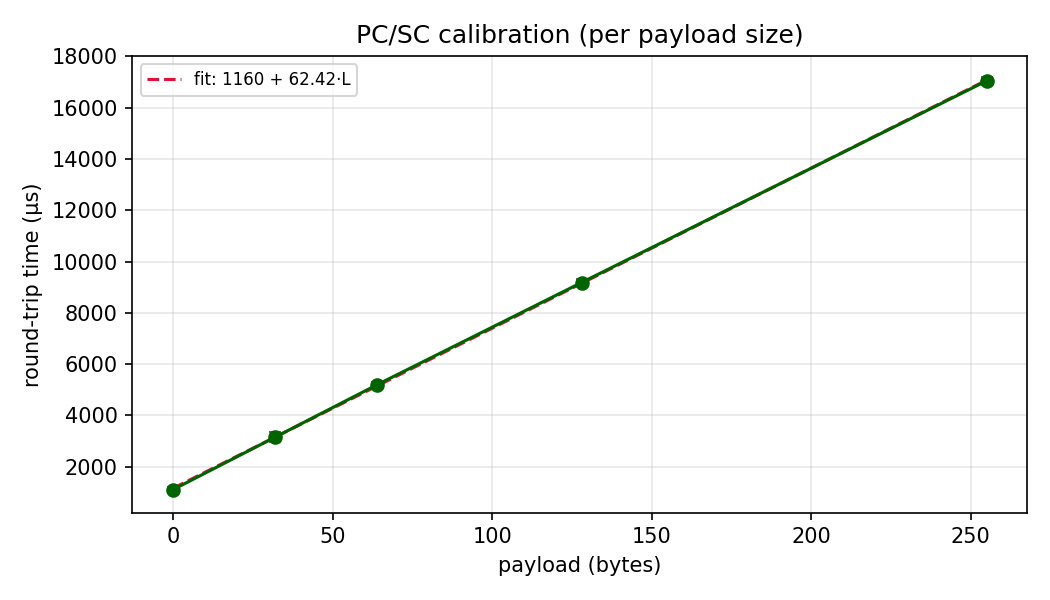
\includegraphics[width=\columnwidth]{pcsc_calibration.png}
\caption{PC/SC overhead model: measured APDU latency versus payload size
  (500 iterations per size). Linear fit with $R^{2} = 0.999$. The
  fitted line is subtracted from all Platform A eUICC timing measurements.}
\label{fig:pcsc-cal}
\end{figure}

\subsection{Hardware-Gap Normalisation}
\label{sec:bench-norm}

Platform A (eUICC) runs classical ECDSA and ECDH operations at firmware
timings; Platform B runs both classical and PQC operations under a known
clock. To project PQC latency from Platform B to the eUICC regime, we
define a per-operation scaling factor:

\begin{equation}
  \alpha_{i} = \frac{T_{\text{eUICC}}(\text{op}_{i})}{T_{\text{PiB}}(\text{op}_{i})}
\end{equation}

\noindent where $T_{\text{eUICC}}(\text{op}_{i})$ is the calibrated
net eUICC computation time for classical operation $\text{op}_{i}$,
and $T_{\text{PiB}}(\text{op}_{i})$ is the corresponding median time
on Platform B. PQC latency on the eUICC is then projected as:

\begin{equation}
  \hat{T}_{\text{eUICC}}(\text{PQC}) = \bar{\alpha} \times T_{\text{PiB}}(\text{PQC})
\end{equation}

The validity of a pooled $\bar{\alpha}$ depends on how uniformly the
two platforms scale across operation types. We evaluate uniformity via
the coefficient of variation $\text{CV} = \sigma(\alpha_i)/\mu(\alpha_i)$
at three hierarchical levels: globally across all classical operations,
within the asymmetric operation family (ECDSA and ECDH), and within the
symmetric operation family (AES-128 and SHA-256). The decision rule,
fixed before data collection, is:

\begin{itemize}[leftmargin=*, noitemsep, topsep=4pt]
  \item $\text{CV}_{\text{global}} \leq 0.10$: use a single pooled
        $\bar{\alpha}$ across all operations; projection error
        is bounded at approximately 10\%.
  \item $\text{CV}_{\text{global}} > 0.10$ but per-family
        $\text{CV} \leq 0.10$: use separate $\bar{\alpha}_{\text{asym}}$
        and $\bar{\alpha}_{\text{sym}}$; PQC signature and KEM
        operations are projected with $\bar{\alpha}_{\text{asym}}$,
        symmetric operations with $\bar{\alpha}_{\text{sym}}$.
  \item Per-family $\text{CV} > 0.10$: use per-operation $\alpha_i$;
        PQC operations with no classical analogue use
        $\bar{\alpha}_{\text{asym}}$ with an additional
        $\pm\text{CV}$ systematic uncertainty bound.
  \item $\text{CV}_{\text{global}} > 0.25$ with no family convergence:
        report Platform B native timings only; linear normalisation is
        deemed unreliable and projections are not made.
\end{itemize}

Projection uncertainty is propagated as:
\begin{equation}
  \sigma_{\hat{T}}^{2} = T_{\text{PiB}}^{2}\,\sigma_{\alpha}^{2} +
  \alpha^{2}\,\sigma_{T_{\text{PiB}}}^{2}
\end{equation}
and all projected values are reported with 95\% confidence intervals.
ARM PMU (Performance Monitoring Unit) cycle counts normalised to the
80 to 200 MHz eUICC clock range provide an independent cross-check of the
projected latencies.

\subsection{Session-Level Results: Classical versus PQ-TLS}
\label{sec:bench-session}

Figure~\ref{fig:session-wall} plots end-to-end session wall time for
all 400 iterations (200 classical TLS, 200 PQ-TLS). Across both modes,
the mean session duration is \textbf{25.20 s} ($\sigma = 0.67$ s).
Table~\ref{tab:session-stats} quantifies the comparison.

\begin{table}[!htb]
\caption{End-to-end session wall time: classical TLS versus PQ-TLS.
  200 successful iterations each. Mean $\pm$ 1$\sigma$.}
\label{tab:session-stats}
\centering
\footnotesize
\setlength{\tabcolsep}{5pt}
\renewcommand{\arraystretch}{1.1}
\begin{tabular}{@{}lrr@{}}
\toprule
\textbf{Mode} & \textbf{Mean (s)} & \textbf{$\sigma$ (s)} \\
\midrule
Classical TLS, configuration (a) & 25.20 & 0.66 \\
PQ-TLS transport, configuration (b) & 25.20 & 0.67 \\
\midrule
Difference & $<$0.01 & n/a \\
\bottomrule
\end{tabular}
\end{table}

A Welch $t$-test yields $p > 0.9$, confirming that the two
distributions are statistically indistinguishable. This result reflects
the dominance of on-card SIM processing time over TLS transport overhead:
the eUICC's AES-128 decryption of the BPP across 18 LoadBPP APDU
operations accounts for approximately 18 s of the 25-second session
budget, leaving the TLS handshake overhead (under 15 ms) negligible
by comparison.

\begin{figure}[!htb]
\centering
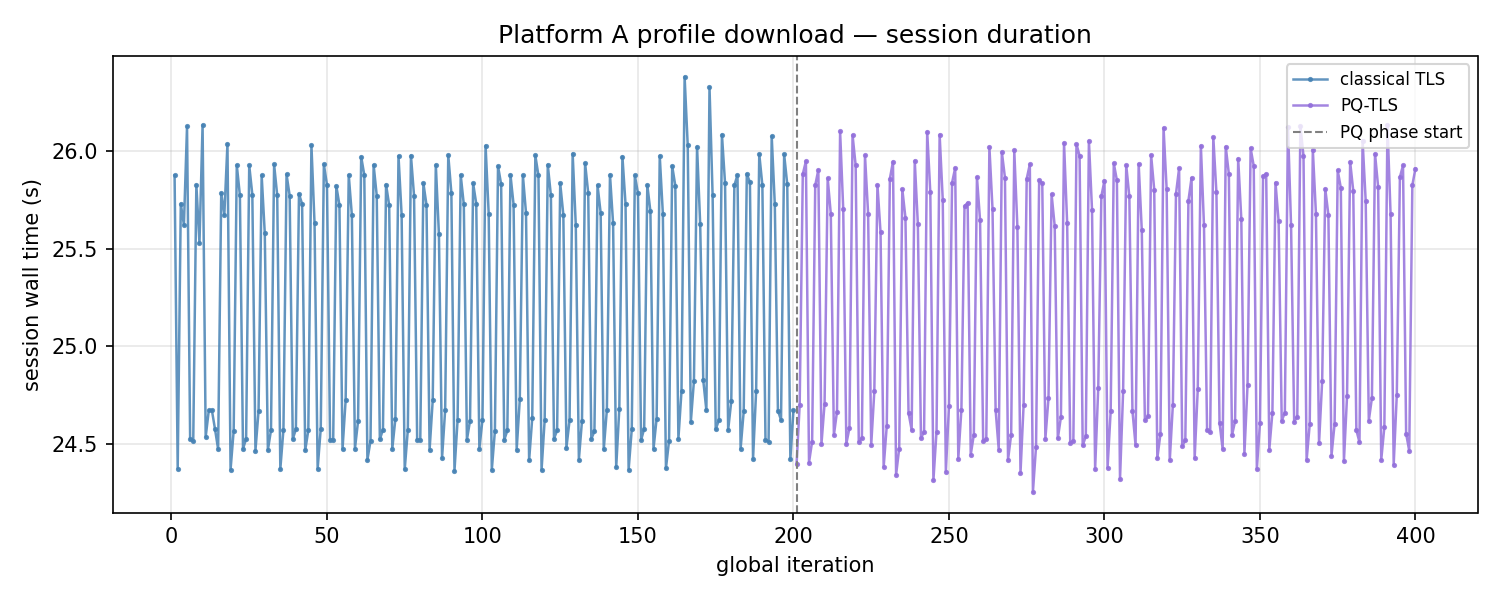
\includegraphics[width=\columnwidth]{session_wall_time.png}
\caption{End-to-end session wall time per iteration. Blue: classical TLS
  (iterations 1 to 200). Purple: PQ-TLS (iterations 201 to 400). The
  dashed vertical line marks the mode transition. Both modes sustain
  approximately 25 s per session with no statistically detectable
  difference.}
\label{fig:session-wall}
\end{figure}

\subsection{Operation-Level Breakdown}
\label{sec:bench-ops}

Figure~\ref{fig:op-means} shows mean per-operation duration averaged
over all 400 iterations. Two APDU commands account for the majority of
cryptographically interesting session time:

\begin{itemize}[leftmargin=*, noitemsep, topsep=4pt]
  \item \texttt{AuthenticateServer} (BF38, step 12): 3,121 ms under
        classical TLS and 3,114 ms under PQ-TLS. This command executes
        ECDSA certificate chain verification and \texttt{serverSigned1}
        verification inside the eUICC; the near-identical times across
        modes confirm that ES9+ transport contributes negligibly.
  \item \texttt{PrepareDownload} (BF21, step 20): 4,075 ms classical,
        4,112 ms PQ-TLS. This command verifies \texttt{smdpSigned2}
        and performs ECDH key generation inside the eUICC.
\end{itemize}

Together, these two commands consume approximately 28\% of the 25-second
session budget. The remaining time is distributed across 18
\texttt{LoadBPP} (BF36) segments, whose cumulative cost of approximately
18 s reflects AES-128 decryption and integrity verification performed
entirely inside the eUICC across the multiple APDU exchanges required to
transfer the full BPP.

\begin{figure}[!htb]
\centering
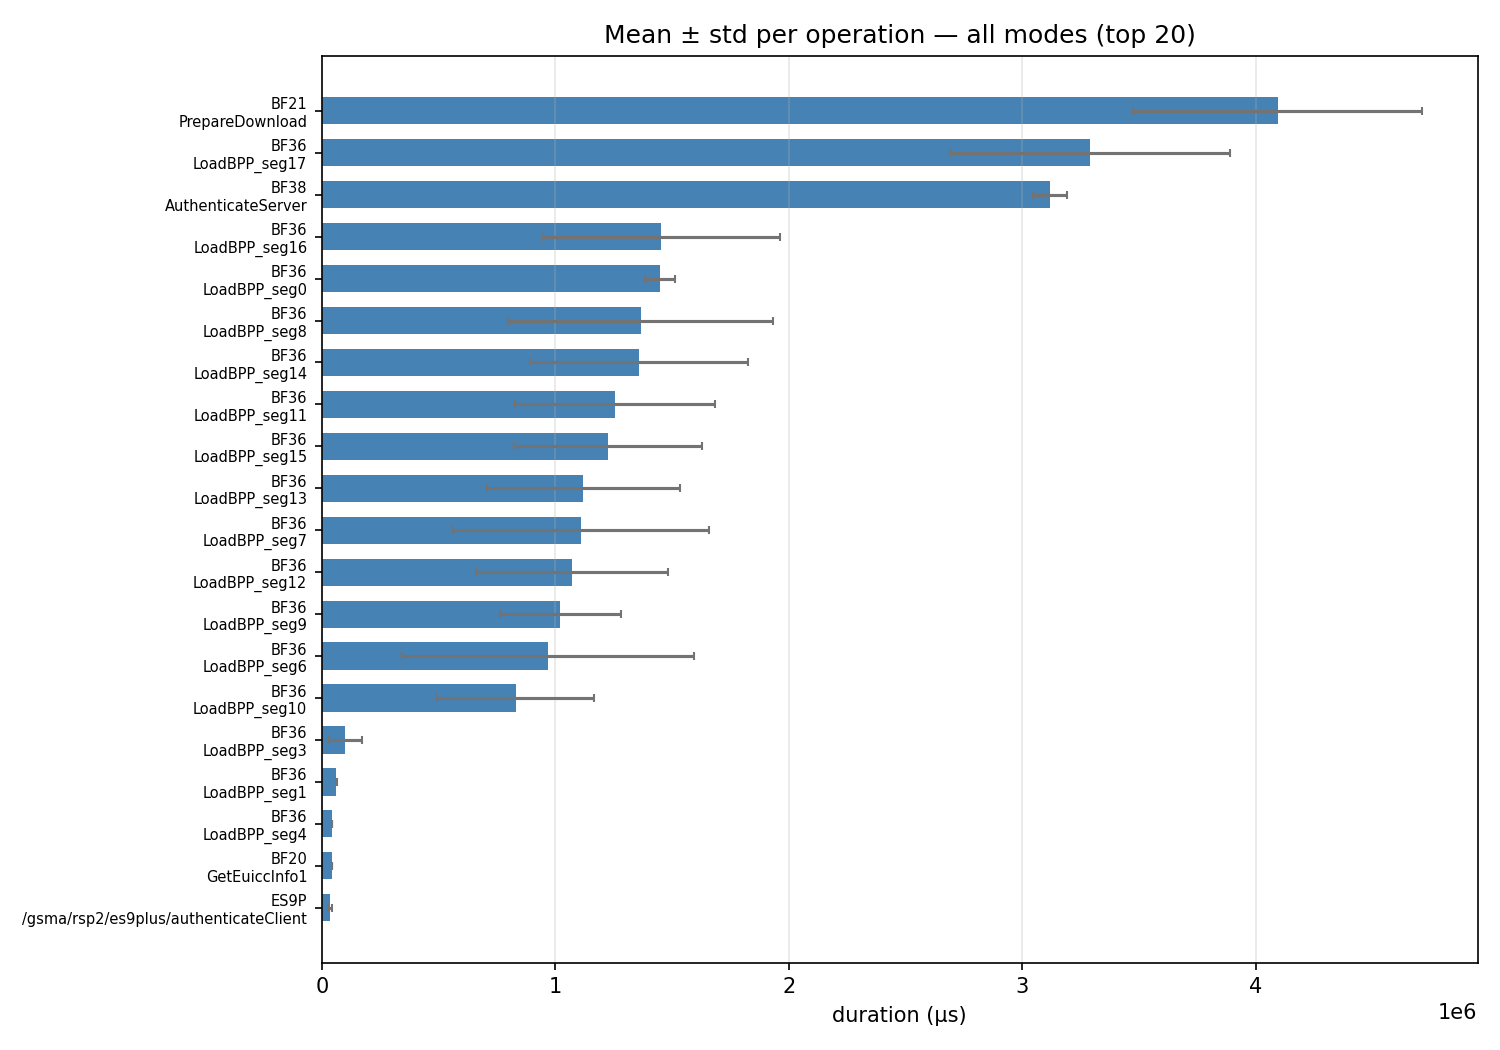
\includegraphics[width=\columnwidth]{operation_means.png}
\caption{Mean APDU and ES9+ operation durations across all 400 iterations.
  On-card APDU operations dominate; ES9+ HTTP calls average below 50 ms
  each and are indistinguishable between classical TLS and PQ-TLS modes.}
\label{fig:op-means}
\end{figure}

The three ES9+ HTTP round-trips (initiateAuthentication,
authenticateClient, and getBoundProfilePackage) each
take between 14 and 37 ms on average and are statistically identical
between classical and PQ-TLS modes (Table~\ref{tab:es9p-times}). TLS
transport cost, even with the larger ML-KEM-768 key exchange messages,
is fully absorbed within this range on a local network.

\begin{table}[!htb]
\caption{ES9+ HTTP call latency: classical TLS versus PQ-TLS. Mean
  over 200 iterations (milliseconds). Although PQ-TLS latencies appear slightly lower across all three calls, the differences are within measurement noise (sub-5~ms on a local network); session-to-session variance accounts for this inversion.}
\label{tab:es9p-times}
\centering
\footnotesize
\setlength{\tabcolsep}{4pt}
\renewcommand{\arraystretch}{1.1}
\begin{tabular}{@{}lrr@{}}
\toprule
\textbf{ES9+ Call} & \textbf{Classical (ms)} & \textbf{PQ-TLS (ms)} \\
\midrule
initiateAuthentication    & 14.7 & 12.2 \\
authenticateClient        & 36.5 & 33.6 \\
getBoundProfilePackage    & 26.4 & 23.8 \\
\bottomrule
\end{tabular}
\end{table}

Per-step latency for ML-DSA-44 sign/verify and ML-KEM-768 encapsulation/decapsulation operations, projected to the eUICC clock domain via the normalisation methodology in Section~\ref{sec:bench-norm}, is reported in Section~\ref{sec:bench-ops} upon completion of Platform B measurements.

\subsection{TLS Handshake Isolation}
\label{sec:bench-tls}

To isolate the bare TLS handshake overhead independent of APDU
processing, we run \texttt{openssl s\_client} in a tight loop (200
iterations per mode) directly against the classical (port 8443) and
PQ-TLS (port 8444) nginx endpoints on the loopback interface.
Figure~\ref{fig:tls-handshake} presents the results.

\begin{figure}[!htb]
\centering
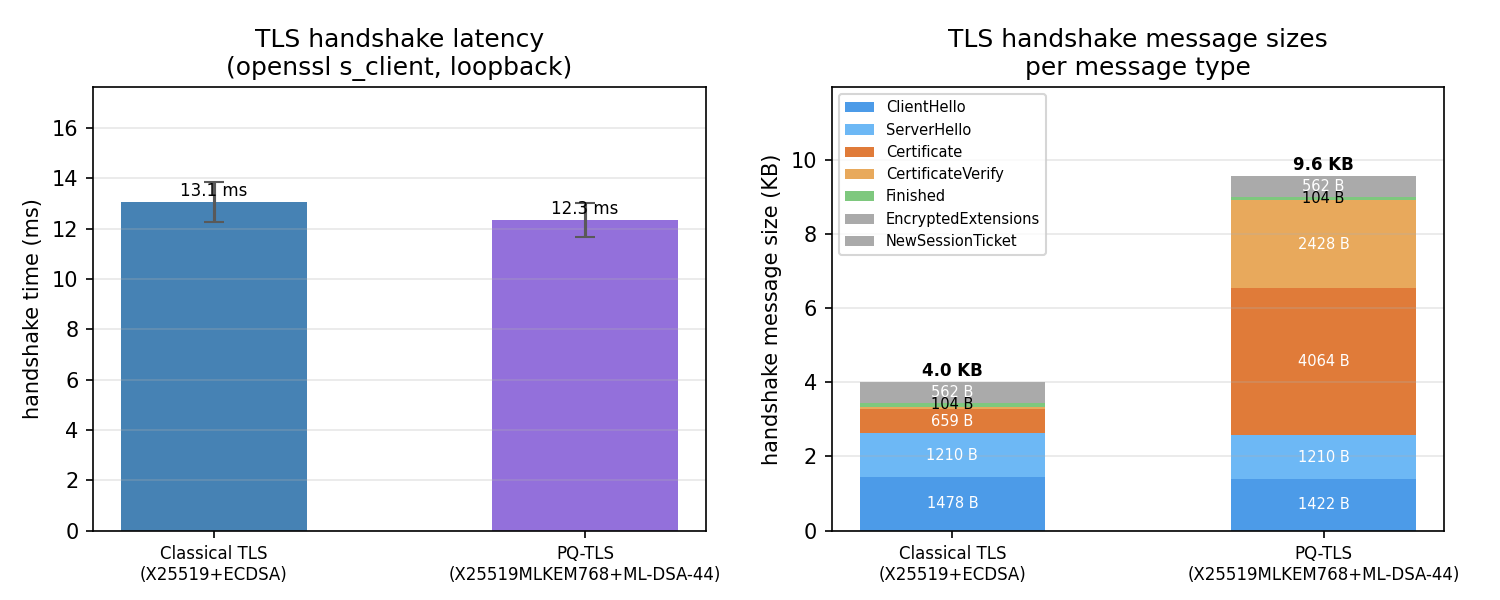
\includegraphics[width=\columnwidth]{tls_handshake.png}
\caption{Left: TLS 1.3 handshake latency measured on the loopback
  interface (200 iterations per mode, mean $\pm$ 95\% CI). Right:
  per-message byte breakdown of the handshake. Classical uses an
  ECDSA-P256 server certificate; PQ-TLS uses an ML-DSA-44 certificate
  with X25519MLKEM768 key exchange.}
\label{fig:tls-handshake}
\end{figure}

Handshake latency is 13.1 ms (classical) versus 12.3 ms (PQ-TLS) on
loopback, within measurement noise. The cost difference lies entirely
in message sizes, not computation:

\begin{itemize}[leftmargin=*, noitemsep, topsep=4pt]
  \item \textbf{Certificate:} 659 B to 4,064 B (factor of 6.2). The
        ML-DSA-44 public key (1,312 bytes) and additional extension
        fields inflate the DER-encoded X.509 leaf certificate.
  \item \textbf{CertificateVerify:} 79 B to 2,428 B (factor of 30.7).
        The ML-DSA-44 signature (2,420 bytes) replaces a 64-byte
        ECDSA-P256 signature value.
  \item \textbf{Total handshake:} approximately 4.1 KB to 9.7 KB
        (factor of 2.4).
\end{itemize}

On a loopback interface transmitting at multi-gigabit rates, the 5.6 KB
increase is negligible in time terms. On a narrowband link such as
100 kbps NB-IoT, the same overhead adds approximately 450 ms per session
establishment, a cost that operators deploying configuration (b) on
constrained IoT ES9+ links must account for in link budget planning.

\subsection{RAM Budget Analysis}
\label{sec:bench-ram}

Table~\ref{tab:ram-budget} models the peak eUICC volatile memory (RAM) requirement during Phase 2 (step 27) against the 9,539 bytes of free memory measured on Platform A. The peak occurs when the long-term identity key (\texttt{SK.EUICC}) and the ephemeral session key (\texttt{otSK.EUICC}) must coexist in memory. Configuration (c) retains a 32-byte ECDSA long-term key alongside the 2,400-byte ML-KEM ephemeral key, requiring 2,432 bytes peak, well within the available budget. Configuration (d) adds the 2,560-byte ML-DSA long-term key, reaching 4,960 bytes peak, but still retains over 4.5~KB of headroom. Both configurations are feasible within current secure-element RAM constraints.

\begin{table}[!htb]
\caption{Peak eUICC volatile memory budget analysis at step 27. \texttt{SK.EUICC} is the long-term identity key; \texttt{otSK.EUICC} is the ephemeral session key. Headroom is calculated against the 9,539~B free RAM measured on Platform A.}
\label{tab:ram-budget}
\centering
\footnotesize
\setlength{\tabcolsep}{4pt}
\renewcommand{\arraystretch}{1.1}
\begin{tabular}{@{}lrrrr@{}}
\toprule
\textbf{Config.} & \textbf{\texttt{SK.EUICC}} & \textbf{\texttt{otSK.EUICC}} & \textbf{Peak Keys} & \textbf{Headroom} \\
\midrule
(a), (b) & 32 B (ECDSA) & 32 B (ECDH) & 64 B & 9{,}475 B \\
(c) & 32 B (ECDSA) & 2{,}400 B (ML-KEM) & 2{,}432 B & 7{,}107 B \\
(d) & 2{,}560 B (ML-DSA) & 2{,}400 B (ML-KEM) & 4{,}960 B & 4{,}579 B \\
\bottomrule
\end{tabular}
\end{table}

\subsection{Certificate Chain Bandwidth Analysis}
\label{sec:bench-bandwidth}

Every SGP.22 provisioning session requires the transmission of two complete X.509 certificate chains (one for the SM-DP+ and one for the eUICC), each comprising four certificates: the CI root, sub-CA, and a leaf pair. Table~\ref{tab:cert-chain} calculates the analytical size of a single application-layer certificate chain across the four configurations. Configurations (a), (b), and (c) use ECDSA certificates and share the same compact chain size. Only configuration (d), which requires ML-DSA-44 CI re-issuance, inflates the chain size by a factor of 6.2, requiring approximately 16.3~KB per chain. This 32.5~KB total session bandwidth increase in configuration (d) underscores the need for robust APDU fragmentation over the constrained ES10c interface.

\begin{table}[!htb]
\caption{Analytical certificate chain size per configuration. Configurations (a), (b), and (c) use ECDSA certificates; configuration (d) uses ML-DSA-44 certificates. Calculations assume a 4-certificate chain with ASN.1/TLV framing overhead included.}
\label{tab:cert-chain}
\centering
\footnotesize
\setlength{\tabcolsep}{4pt}
\renewcommand{\arraystretch}{1.1}
\begin{tabular}{@{}lrrr@{}}
\toprule
\textbf{Configuration} & \textbf{Per-Cert Size} & \textbf{Chain Size (4 certs)} & \textbf{Factor} \\
\midrule
(a), (b), (c) & 659 B & 2{,}636 B & 1.0$\times$ \\
(d)           & 4{,}064 B & 16{,}256 B & 6.2$\times$ \\
\bottomrule
\end{tabular}
\end{table}

\subsection{Configuration (b) Overhead Summary}
\label{sec:bench-summary}

Table~\ref{tab:option-b-summary} consolidates the measured configuration
(b) overhead relative to the classical baseline across all measured
dimensions.

\begin{table}[!htb]
\caption{Configuration (b) overhead summary: PQ-TLS transport with
  classical application-layer cryptography. Loopback measurements;
  200 iterations each.}
\label{tab:option-b-summary}
\centering
\footnotesize
\setlength{\tabcolsep}{4pt}
\renewcommand{\arraystretch}{1.1}
\begin{tabular}{@{}lrrr@{}}
\toprule
\textbf{Metric} & \textbf{Classical} & \textbf{PQ-TLS} & \textbf{Factor} \\
\midrule
Session wall time (s)        & 25.20 & 25.20 & 1.00 \\
TLS handshake latency (ms)   & 13.1  & 12.3  & 0.94 \\
TLS total message size (KB)  & 4.1   & 9.7   & 2.37 \\
Certificate size (B)         & 659   & 4{,}064 & 6.16 \\
CertificateVerify (B)        & 79    & 2{,}428 & 30.7 \\
\bottomrule
\end{tabular}
\end{table}

The central finding is that configuration (b) imposes zero measurable
latency overhead on end-to-end RSP sessions. The approximately 5.6 KB
increase in TLS handshake bytes is absorbed entirely within the dominant
on-card SIM processing time. The real deployment cost of configuration (b)
is therefore bandwidth-bound, not computation-bound, and is relevant only
for low-throughput ES9+ links.

% =======================================================================
%  SECTION 7: DISCUSSION
% =======================================================================
\section{Discussion}
\label{sec:discussion}

\subsection{Synthesis of Verification and Benchmark Results}
\label{sec:disc-synthesis}

The formal verification and benchmark results together provide a coherent
picture of the four migration configurations. Configuration (a) is the
fully classical baseline: all six security properties hold under the
Dolev-Yao model, but Q3, Q4, and Q6 collapse under the quantum attacker.
This is the status quo for all deployed Consumer RSP installations.
Configuration (b) is immediately deployable as a purely server-side
upgrade and provides zero measurable latency cost on end-to-end RSP
sessions; however, its role is transport-level mitigation only. As the
formal verification confirms, it does not address the application-layer
ECDH exposure: the eUICC-to-LPA channel carries both ephemeral EC public
keys in plaintext, making the Shor oracle applicable regardless of ES9+
TLS mode, and leaving configuration (b) equivalent to (a) against an
HNDL adversary who can observe the local interface.

Configuration (c) replaces ECDH with ML-KEM-768 for session key
agreement while retaining ECDSA for authentication and the existing CI
trust hierarchy. This is sufficient to close Q3, Q4, and Q6 under the
quantum attacker: with no ECDH types in the model, the Shor oracle is
vacuously inapplicable. The HNDL threat on session key confidentiality
is eliminated with the smallest possible deployment footprint: no CI
re-issuance, ECDSA certificate chains unchanged, silicon requirement
limited to ML-KEM-768 only. The residual quantum threat to ECDSA
authentication (forgery by a live CRQC at session time) is addressed in
configuration (d) by additionally replacing ECDSA with ML-DSA-44,
achieving full application-layer quantum resistance at the cost of CI
re-issuance, enlarged ML-DSA-44 certificate chains, and more demanding
silicon requirements.

From a performance perspective, configurations (c) and (d) share the
ML-KEM-768 operation timings for steps 21a, 24b, and 27b. The incremental
computational cost of configuration (d) over (c) isolates ML-DSA-44
authentication overhead: four sign/verify operations in Phase 1 and three
in Phase 2, plus two full ML-DSA-44 CI certificate chain transmissions.
Preliminary per-operation measurements indicate that ML-DSA-44 signing is
significantly more computationally expensive than ECDSA-P256 signing on
constrained hardware, and the certificate chain size inflation in
configuration (d) will require APDU fragmentation support in the SGP.22
APDU layer.

\subsection{Phased Migration Outlook}
\label{sec:disc-migration}

Based on verification and benchmark results, we recommend a three-phase
migration approach driven by distinct threat motivations:

\textbf{Phase 1 (deployable now): Configuration (b).} SM-DP+ operators
should upgrade their ES9+ TLS endpoints to support X25519MLKEM768 and
ML-DSA-44 certificates, and require PQ-TLS from LPA clients. This
requires only server-side software updates and an LPA update; no eUICC
modification is needed. Configuration (b) provides transport-level HNDL
mitigation for the ES9+ channel and establishes the operational
infrastructure for subsequent phases. It does not close the
application-layer ECDH exposure; that requires configuration (c).
Operators on constrained ES9+ links (below 1 Mbps) should perform link
budget analysis for the 5.6 KB handshake overhead.

\textbf{Phase 2 (HNDL closure, next silicon generation): Configuration (c).}
When new eUICC silicon incorporating ML-KEM-768 becomes available,
operators should plan refresh cycles to deploy configuration (c) for new
device activations. This closes the HNDL threat on session key
confidentiality without CI re-issuance: only SGP.22 specification updates
for the ML-KEM-768 algorithm identifier in \texttt{euiccInfo1} and
\texttt{euiccInfo2} and the structural change to \texttt{bind\_body} are
required. Configuration (c) should be prioritised over (d) for near-term
deployment because the two quantum threats operate on asymmetric timelines:
HNDL attacks on session-key confidentiality can be executed offline from
recorded traffic today, while ECDSA forgery requires a live CRQC present
at session time. Closing the offline threat first, with the smallest possible
deployment footprint, is therefore the rational sequencing.

\textbf{Phase 3 (full quantum resistance): Configuration (d).} When
eUICC silicon supporting both ML-DSA-44 and ML-KEM-768 is available,
new device activations should use configuration (d) for complete
application-layer quantum resistance. This additionally requires CI root
re-issuance with ML-DSA-44 keys, SGP.22 specification updates for PQC
algorithm identifiers, and APDU fragmentation support for enlarged
ML-DSA-44 certificate chains.

The NSA CNSA 2.0 mandate (2035)~\cite{nsa_cnsa2} implies that devices
manufactured today with typical five-year lifetimes will still be active
past the deadline. Operators should treat configuration (b) as an
immediate baseline, prioritise configuration (c) for the next eUICC
silicon generation to close the HNDL window, and plan configuration (d)
for full quantum resistance in alignment with GSMA PQ.04~\cite{gsma_pq04}
and NIST IR 8547~\cite{nist_ir8547}.

\subsection{Limitations and Future Work}
\label{sec:disc-limitations}

This evaluation has several limitations that future work should address.
First, Platform B (ARM Cortex-A53 at 1 GHz) is used as a proxy for eUICC
PQC performance; the normalisation methodology introduces uncertainty
that is propagated and bounded but not eliminated. Direct measurements
on PQC-capable eUICC silicon, once available, would replace projected
values with ground-truth timings.

Second, the formal verification uses the symbolic Dolev-Yao model, which
treats cryptographic primitives as perfect black boxes. A computational
security analysis would provide stronger guarantees but is significantly
more complex to apply to a protocol of this size. The symbolic model
is nonetheless widely accepted for protocol security analysis and
captures the key structural properties of interest.

Third, this evaluation covers ML-KEM-768 and ML-DSA-44 specifically.
Other NIST Level 3 and Level 2 candidates (including SLH-DSA and
BIKE) could in principle be evaluated in the same framework; comparison
with alternative PQC candidates is left for future work.

Fourth, the evaluation does not cover hybrid key agreement modes, which
would combine classical ECDH with ML-KEM-768 in a single session to
preserve a classical security hedge. Hybrid modes would provide defence
in depth if ML-KEM lattice assumptions are later weakened, at the cost
of larger message sizes and more complex protocol state. Evaluation of
hybrid KA alongside configuration (c) is deferred to future work.

Fifth, the evaluation does not cover hybrid certificate formats, which
may be desirable during the transition period to maintain backward
compatibility with eUICCs that do not support PQC. Hybrid modes
(combining ECDSA and ML-DSA in a single certificate or chain) would
require additional ASN.1 encoding analysis and protocol modifications.

Sixth, the SGP.22 APDU fragmentation layer has not been stress-tested
with the larger certificate chain sizes required by configuration (d).
APDU chunking behaviour and error recovery under fragmented ML-DSA-44
certificate chains is an important implementation concern for eUICC
vendors. Configuration (c) retains ECDSA certificate sizes and is not
affected by this concern.

Seventh, the analysis assumes an honest passive LPA (Section~\ref{sec:sys-threat},
assumption~T3). A compromised LPA that rewrites application-layer
messages, injects traffic, or terminates TLS dishonestly falls outside
the model: such an adversary must be treated as a separate trust failure
and is not covered by the verification results here.

% =======================================================================
%  SECTION 8: CONCLUSION
% =======================================================================
\section{Conclusion}
\label{sec:conclusion}

This paper has presented a comprehensive evaluation of post-quantum
cryptography migration for GSMA SGP.22 Consumer Remote SIM Provisioning,
combining formal protocol verification with hardware benchmarking across
four incremental migration configurations.

The formal verification using ProVerif 2.05 confirms that the six
security properties analysed in this study for SGP.22 hold across all
four configurations under the standard Dolev-Yao adversary model, validating the correctness of the
protocol logic independently of algorithm strength. Under a
quantum-enhanced adversary equipped with a Shor oracle modelling the
HNDL threat, session key secrecy (Q3), profile confidentiality (Q4),
and forward secrecy (Q6) collapse for configurations (a) and (b), while
all six properties hold for configurations (c) and (d). Authentication
properties (Q1, Q2) pass in all configurations in this scoped model because
the oracle is intentionally limited to ECDH key-agreement inversion and does
not grant ECDSA forgery; under a complete Shor adversary including ECDSA
forgery, only configuration~(d) retains all six properties. In practice,
Shor's algorithm also breaks ECDSA, which is addressed separately by
configuration (d). This two-tier
outcome is the key formal result: ML-KEM-768 key agreement in
configuration (c) closes the HNDL exposure on session-key secrecy and
profile confidentiality within the analysed model, with the Shor oracle
vacuously inapplicable due to the absence of ECDH types.
Configuration (c) achieves this without CI re-issuance and with a minimal
silicon footprint (ML-KEM-768 only), making it the highest-priority
deployment target for closing the HNDL exposure window. Configuration (d)
adds ML-DSA-44 authentication for full quantum resistance, at the cost of
CI re-issuance and enlarged ML-DSA-44 certificate chains.

The benchmark results demonstrate that configuration (b) is immediately
deployable with zero measurable impact on end-to-end RSP session latency
(25.20 s mean in both modes, $p > 0.9$). TLS handshake message size
increases by a factor of 2.4 (from approximately 4.1 KB to 9.7 KB),
with the CertificateVerify field increasing by a factor of 30.7 due to
the ML-DSA-44 server certificate. On broadband ES9+ links this overhead
is negligible; on constrained links below 1 Mbps, operators should
perform link budget analysis. Configurations (c) and (d) require new
eUICC silicon and SGP.22 specification updates; configuration (d)
additionally requires CI root re-issuance and APDU fragmentation support.
Based on our hardware-gap normalisation, the anticipated performance
impact of configuration (d) on eUICC computation time is dominated by
ML-DSA-44 signature verification in the mutual authentication phase.

The combined results support a phased migration strategy: deploy
configuration (b) immediately as a transport-level HNDL mitigation for
ES9+ transport (noting that it does not address the application-layer
ECDH exposure), prioritise configuration (c) for the next eUICC silicon
generation to close the HNDL window on session keys, and target
configuration (d) for full application-layer quantum resistance aligned
with the NSA CNSA 2.0 mandate by 2035.

\section*{Acknowledgment}
The authors thank the open-source maintainers of osmo-smdpp and the Open
Quantum Safe project for making their implementations publicly available.

\clearpage
\bibliographystyle{model1-num-names}
\bibliography{cas-refs}

\end{document}
